\documentclass[12pt, twoside, a4paper]{report}

\usepackage[LGR, T1]{fontenc}
\usepackage[utf8]{inputenc}
\usepackage[english,greek]{babel}
\usepackage{alphabeta}
\newcommand{\en}[1]{\selectlanguage{english}#1\selectlanguage{greek}}

\usepackage{graphicx}
\usepackage{float}

\usepackage{listings}
\renewcommand*{\lstlistingname}{\en{Code}}
\lstset{
	language=C,                % choose the language of the code
	numbers=left,                   % where to put the line-numbers
	stepnumber=1,                   % the step between two line-numbers.
	numbersep=5pt,                  % how far the line-numbers are from the code
}

\usepackage{url}
\newcommand{\itt}[1]{\textit{#1}}


\begin{document}

%%Title
\title{
\vspace{-6ex}
\begin{center}

\includegraphics[scale=1]{pyrforos.eps}
\end{center}
\Large{Ε}\large{ΘΝΙΚΟ}
\Large{Μ}\large{ΕΤΣΟΒΙΟ}
\Large{Π}\large{ΟΛΥΤΕΧΝΕΙΟ} \\
\normalsize{Τ}\small{ΜΗΜΑ}
\normalsize{Η}\small{ΛΕΚΤΡΟΛΟΓΩΝ}
\normalsize{Μ}\small{ΗΧΑΝΙΚΩΝ}
\normalsize{Κ}\small{ΑΙ}
\normalsize{Μ}\small{ΗΧΑΝΙΚΩΝ}
\normalsize{Υ}\small{ΠΟΛΟΓΙΣΤΩΝ} \\
\vspace{2ex}
ΤΟΜΕΑΣ ΠΛΗΡΟΦΟΡΙΚΗΣ ΚΑΙ ΥΠΟΛΟΓΙΣΤΩΝ \\
ΕΡΓΑΣΤΗΡΙΟ ΥΠΟΛΟΓΙΣΤΙΚΩΝ ΣΥΣΤΗΜΑΤΩΝ \\
\vspace{8ex}
\large \textbf{Υλοποίηση \en{utmem (Userspace Transcedent Memory)} ως \en{unikernel}} \\
\vspace{10ex}
\large
ΔΙΠΛΩΜΑΤΙΚΗ ΕΡΓΑΣΙΑ \\
\vspace{2ex}
\normalsize
του \\
\vspace{2ex}
\parbox[c]{0.8\textwidth} { \center\textbf{
Ιωάννη Αραβαντινού-Σιμωνέτου }}

\vspace{10ex}
\flushleft
\begin{tabbing}
	\textbf{Επιβλέπων}: \= -Εισάγετε το όνομα, αρχικό πατρωνύμου
				και επίθετο- \\
			    \> -Εισάγετε τον τίτλο του επιβλέποντα-
\end{tabbing}
}

%%Date
\date{
\normalsize
Αθήνα, -Εισάγετε το μήνα και το έτος κατάθεσης της εργασίας-}

\maketitle
\newpage
\hspace{10pt}
%\tiny
%(this page is left intentionally blanc)
%\normalsize
\newpage

\includegraphics{pyrforos.eps}
\noindent
\parbox[b]{0.8\textwidth} {\textbf{
\noindent
\normalsize{Ε}\small{ΘΝΙΚΟ}
\normalsize{Μ}\small{ΕΤΣΟΒΙΟ}
\normalsize{Π}\small{ΟΛΥΤΕΧΝΕΙΟ}} \\
\small
ΤΜΗΜΑ
ΗΛΕΚΤΡΟΛΟΓΩΝ
ΜΗΧΑΝΙΚΩΝ
ΚΑΙ
ΜΗΧΑΝΙΚΩΝ
ΥΠΟΛΟΓΙΣΤΩΝ \\
-ΕΙΣΑΓΕΤΕ ΤΟΝ ΤΟΜΕΑ- \\
-ΕΙΣΑΓΕΤΕ ΤΟ ΕΡΓΑΣΤΗΡΙΟ-
}

%new page
\begin{center}
\vspace{8ex}
\large \textbf{-Εισάγετε τον τίτλο της διπλωματικής εργασίας-} \\
\vspace{10ex}
\large
ΔΙΠΛΩΜΑΤΙΚΗ ΕΡΓΑΣΙΑ \\
\vspace{2ex}
\normalsize
-Εισάγετε το σωστό άρθρο (της/του/των)- \\
\vspace{2ex}
\parbox[c]{0.4\textwidth} { \center\textbf{
-Εισάγετε το όνομα, αρχικό πατρώνυμου και επωνυμο των συγγραφέων- }}
\parbox[c]{0.4\textwidth} { \center\textbf{
	-another author, whose name is here- }}
\vspace{10ex}
\flushleft
\begin{tabbing}
\textbf{Επιβλέπων}: \= -Εισάγετε το όνομα, αρχικό πατρωνύμου
			και επίθετο- \\
		    \> -Εισάγετε τον τίτλο του επιβλέποντα-
\end{tabbing}
\end{center}


\noindent
Εγκρίθηκε από την τριμελή εξεταστική επιτροπή την -εισάγετε ημερομηνία-.

\begin{center}
\scriptsize
\parbox[b]{0.3\textwidth} {\center
	........................................
	-Εισάγετε ονοματεπώνυμο-
	-Εισάγετε τίτλο-
}
\parbox[b]{0.3\textwidth} {\center
	........................................
	-Εισάγετε ονοματεπώνυμο-
	-Εισάγετε τίτλο-
}
\parbox[b]{0.3\textwidth} {\center
	........................................
	-Εισάγετε ονοματεπώνυμο-
	-Εισάγετε τίτλο-
}
\end{center}
\vspace{10ex}
\normalsize
\noindent
Αθήνα, (εισάγετε το μήνα και το έτος κατάθεσης της εργασίας).
\newpage
\hspace{10pt}

\vspace{30ex}
\noindent
................................... \\
\textbf{(Εισάγετε όνομα, αρχικό πατώνυμου και επίθετο συγγραφέα)} \\
(Εισάγετε τον απονεμηθέντα τίτλο στο συγγραφέα) \\
\vspace{8ex}


\vspace{50ex}

\small
\noindent
\copyright \hspace{1em}(Εισάγετε έτος έκδοσης) Εθνικό Μετσόβιο Πολυτεχνείο.
All rights reserved.



\begin{abstract}
Με την σταδιακή μετακίνηση της επεξεργασίας των δεδομένων και την
εκτέλεση των εφαρμογών από τοπικά υπολογιστικά συστήματα σε
εικονικοποιημένα \en{cloud} συστήματα, γίνεται εμφανές πως τα συμβατικά
λειτουργικά συστήματα αδυνατούν να επιτελέσουν αποδοτικά τον ρόλο τους.
Σχεδιασμένο δεκαετίες πριν, ένα συμβατικό λειτουργικό σύστημα εισάγει
περιττές εξαρτήσεις, αυξημένες ανάγκες σε υπολογιστικούς πόρους και
χρονικές επιβαρύνσεις κατά την \en{cloud} εκτέλεση του. Η τεχνολογία
των \en{unikernel}, στοχεύει στην εξάλειψη των ανώτερων προβλημάτων,
δημιουργώντας μια ελαφριά, εξειδικευμένη και ταχύτατη εικονική
μηχανική, η οποία στοχεύει στην εκτέλεση μιας μοναδικής λειτουργίας,
και που ταιριάζει καλύτερα στο \en{cloud περιβάλλον}. Ταυτόχρονα, η
εικονικοποίηση των υπολογιστικών συστημάτων οδηγεί αναπόφευχτα σε υποβέλτιστη
χρησιμοποίηση των διαθέσιμων πόρων, και ειδικά της μνήμης. Ο
μηχανισμός ελαστικής μνήμης \en{utmem} εκμεταλλεύεται την συνεργασίας
του εικονικοποιημένου συστήματος και του επόπτη, επιτρέποντας
την παραεικονοποίηση, με σκοπό την αυξημένη απόδοση χρήσης της
μνήμης από τις εικονικοποιημένες εφαρμογές. Σκοπός της παρούσας
εργασίας, είναι η μελέτη των χαρακτηριστικών και της φιλοσοφίας
διάφορων \en{unikernel} περιβάλλοντων, καθώς και του μηχανισμού της
\en{utmem} με τελικό στόχο την ενσωμάτωση του τελευταίου σε κάποιο
\en{unikernel} περιβάλλον. Τέλος, αποτιμάται πειραματικώς η χρηστική αξία του εν λόγω συνδυασμού
των δύο αυτών καινοτόμων τεχνολογιών, ως προς συμβατικά περιβάλλοντα
εικονικοποίησης και περιβάλλοντα \en{lightweight} εικονικοποίησης.
\end{abstract}

\newpage
\renewcommand{\abstractname}{\en{Abstract}}

\begin{abstract}
\en{
The gradual transition of data processing and application execution, from local
computer system to virtualized cloud systems, makes apparent that conventional
operating systems are unable to fulfill their role effectively. Designed
decades ago, a conventional operating system introduces superfluous
dependencies, increased needs in computational resources and temporal
delays when executed on the cloud. The technology of unikernel aims to the
elimination of the aforementioned problems, by creating a lightweight,
specialized and fast virtual machine, which supports execution of a unique
function, and which fits better on the cloud environment. Meanwhile, the
virtualization of computer system inevitably leads to suboptimal usage of the available
resources, especially that of memory. The elastic memory mechanism utmem
takes advantage of the cooperation between the virtualized system and the
hypervisor, allowing paravirtualization techniques, in purpose to elevate
efficiency of memory used by virtualized applications. The goal of this
thesis is the study of the philosophy and the characteristics of various
unikernel frameworks, as well as the mechanism of utmem, with ultimate
cause the incorporation of the latter to a unikernel environment. Finally,
the functional value of that innovative technologies' combination is
evaluated, in aspect of both conventional virtualization environments and
lightweight virtualization environments.
}
\end{abstract}



\tableofcontents

\listoffigures


\chapter{Εισαγωγή}

Με την αυγή της τρίτης δεκαετίας του εικοστού πρώτου αιώνα, έχει καταστεί
σαφές πως οι υπηρεσίες του \en{cloud computing} αποτελούν ένα από τα
ισχυρότερα εργαλεία της σύγχρονης τεχνολογίας των υπολογιστών. Ως εκ τούτου,
αποτελεί αντικείμενο σχολαστικής μελέτης από πανεπιστημιακά ιδρύματα και
ερευνητικά κέντρα παγκοσμίως.
Ο όρος \en{cloud computing} αναφέρεται σε ένα αφηρημένο μοντέλο υπολογιστικών δομών ανεξάρτητό
από τα φύσικό υλικό (\en{hardware}) όπου γίνονται οι υπολογισμοί, σε αντίθεση με τα παραδοσιακά
\en{IT infrastructure} όπου το υλικό είναι άμεσα προσβάσιμο και αλληλένδετο με την εκάστοτε
επεξεργαστική δραστηριότητα.
Το μεγάλο πλεονέκτημα του \en{cloud computing},
είναι η \en{on-demand} πρόσβαση σε υπηρεσίες ή και υπολογιστικούς
πόρους χωρίς την άμεση εμπλοκή της χρήστη, από απομακρυσμένο περιβάλλον\cite{wikipediaCloud}.
\newline

Το \en{cloud computing} στηρίζεται σε μεγάλο βαθμό στην εικονικοποίηση (\en{virtualization}).
Με τον όρο εικονικοποίηση περιγράφεται η διαδικασία εκτέλεσης ενός εικονικού
(σε αντιδιαστολή με το πραγματικό) στιγμιοτύπου ενός υπολογιστικού συστήματος, σε
αφαίρεση από το πραγματικό υλικό επάνω στο οποίο γίνεται η εκτέλεση.
Υπάρχουν διάφορα είδη εικονικοποίησης. Ένα αρκετά γνωστό στον μέσο προγραμματιστή
είδος είναι η εικονικοποίηση σε επίπεδο εφαρμογών, όταν η γλώσσα
προγραμματισμού επιβάλει την εκτέλεση της εφαρμογής εντός εικονικού περιβάλλοντος,
π.χ. η \en{java} με το \en{JVM}\cite{JVM}. Ένα στιγμιότυπο εικονικοποίησης και προσομοίωσης
ενός υπολογιστικού συστήματος ονομάζεται εικονική μηχανή (\en{virtual machine} ή \en{VM}).
Η παρούσα διπλωματική εργασία ασχολείται με την εικονικοποίηση σε επίπεδο
συστήματος, όπου το σύνολο του υλικού του συστήματος εικονικοποιείται με την
βοήθεια κάποιου επόπτη (\en{hypervisor}). Τέτοιοι επόπτες είναι συνήθως το \en{KVM},
το \en{Xen} κ.α.
\newline
\begin{figure}[h]
  
\includegraphics[width=0.7\textwidth]{pictures/generalVirtulization.png}
  \caption{Παραδοσιακό σύστημα και Εικονοποιημένο σύστημα}
  \label{fig:generalVirtulization}
\end{figure}

Ο επόπτης είναι ένα σύνολο λογισμικού, το οποίο επιτρέπει την
εικονικοποίηση ενός συστήματος. Οι εποπτές μπορεί να είναι διεργασίες-μέρη ενός άλλου λειτουργικού συστήματος (\en{host})
ή να παρεμβάλλονται απευθείας ανάμεσα στο υλικό και το εικονοποιημένο σύστημα
(\en{guest}). Στην πρώτη περίπτωση ονομάζονται επόπτες τύπου II, ενώ στην δεύτερη
επόπτες τύπου I\cite{Aimilios}.
\newline
\begin{figure}[h]
  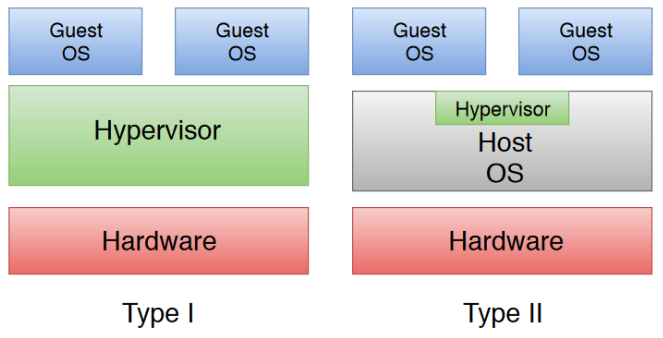
\includegraphics[width=0.7\textwidth]{pictures/typeI-II-hypervisors.PNG}
  \caption{Επόπτες τύπου I και τύπου ΙΙ}
  \label{fig:typeI-II}
\end{figure}


Ταυτόχρονα με την εικονικοποίηση, χρησιμοποιείται και τεχνική της προσομοίωσης
(\en{emulation}). Με την προσομοίωση, μπορεί να αναπαραχθεί πιστά η συμπεριφορά ενός
κομματιού υλικού, το οποίο δεν έχει κάποιο φυσικό αντίστοιχο στο υφιστάμενο πραγματικό
σύστημα. Τέτοια κομμάτια υλικού μπορεί να είναι, για παράδειγμα, μια κάρτα δικτύου. Η
αναπαραγωγή της συμπεριφοράς γίνεται εξ ολοκλήρου σε επίπεδο λογισμικού
(\en{software}). Ένα ευρέως διαδεδομένο πρόγραμμα προσομοίωσης είναι
το \en{QEMU (Quick EMUlator)},
το οποίο μπορεί να λειτουργήσει και ως επόπτης, ενώ ο συνδυασμός \en{emulator-hypervisor}
\en{QEMU/KVM} είναι
μια από τις αποτελεσματικότερες λύσεις για εικονικοποίηση της εκτέλεσης ενός
λειτουργικού συστήματος\cite{QemuWiki}.

\section{Είδη εικονικοποίησης}

Με την πλήρη εικονικοποίηση, προσομοιώνεται η λειτουργία ενός πλήρους λειτουργικού
συστήματος. Μια σημαντική ιδιότητα είναι πως δεν υπάρχει υποβοήθηση από το
υλικό \en{(hardware assisted)}, όπως εμφανίζεται σε άλλη περίπτωση στην συνέχεια.
Το λειτουργικό σύστημα που προσομοιώνεται (\en{guest}) δεν χρειάζεται να υποστεί
καμία αλλαγή και προσφέρεται ως έχει. Ο \en{hypervisor} προσφέρει οτιδήποτε
χρειάζεται ο \en{guest} σε επίπεδο υλικού, έτσι ώστε ο \en{guest} να αισθάνεται πως
εκτελείται επάνω σε πραγματικό υλικό, όπως είναι σχεδιασμένος να κάνει.
Ταυτόχρονα, προσομοιώνει και την εκτέλεση των εντολών του επεξεργαστή.
Ειδική μνεία χρειάζεται για τις προνομιούχες εντολές του \en{guest}, οι οποίες
δεν επιτρέπεται για λόγους ασφάλειας να εκτελεστούν απευθείας επάνω στην
\en{CPU}, και για αυτό τον λόγο εφαρμόζονται διαφορετικές λύσεις όπως η \en{trap and
emulate}. Μάλιστα, ειδικά για την \en{x86} αρχιτεκτονική, η δυσκολία στο να
προσομοιωθούν αυτές οι συγκεκριμένες εντολές έκαναν αρχικά την εικονικοποίηση να μοιάζει
αδύνατη \cite{VMwarePaper}.
\newline

H προηγούμενη τεχνική έχει το μειονέκτημα της μειωμένης ταχύτητας εκτέλεσης.
Για τον λόγο αυτό έχει αναπτυχθεί η εικονικοποίηση με υποβοήθηση υλικού
(\en{hardware assisted virtualization}), όπου έχουν προστεθεί εντολές στην \en{CPU},
οι οποίες βοηθούν την εκτέλεση του συνόλου των εντολών του \en{guest}, δίχως
μείωση  στην ταχύτητα. Και σε αυτήν την περίπτωση ο \en{guest} εκτελείται ως
έχει, χωρίς κάποια τροποποίηση, όμως υπάρχει πρόβλεψη από το υλικό ώστε να
επιταχύνει την εκτελεσή του με ασφάλεια\cite{VMwarePaper}. Αυτή η τεχνική είναι διαθέσιμη
εφόσον υπάρχουν επεκτάσεις υλικού (\en{virtualization extensions}), όπως η
τεχνολογία \en{VT-x} της \en{Intel} και \en{AMD-V} της \en{AMD} στους επεξεργαστές της εκάστοτε εταιρείας\cite{wikipediaX86}.
\newline

Επιπροσθέτως, η άγνοια του \en{guest}, ως προς την εκτέλεση του επάνω σε εικονικό
σύστημα, μπορεί μεν είναι μια πολύ επιθυμητή αφαίρεση, οδηγεί όμως συχνά σε
μη βέλτιστη συμπεριφορά και χρήση των πόρων του πραγματικού συστήματος. Για
παράδειγμα η διαχείριση της υφιστάμενης μνήμης \en{RAM}, δεν γίνεται με βέλτιστο
τρόπο, από μεριάς \en{guest}, καθώς δεν γνωρίζει πραγματικά πόση συνολικά διαθέσιμη
υπάρχει στο σύστημα, παρά μόνο τόση όση έχει ανατεθεί από τον \en{host} στον
\en{guest}.  Με την παρα-εικονικοποίηση (\en{paravirtualization}), ο \en{guest} γνωρίζει
πως δεν εκτελείται επάνω σε φυσικό σύστημα, και ζητά την συνεργασία του
επόπτη του για την αποδοτικότερη αντιμετώπιση συγκεκριμένων σεναρίων χρήσης
του. Επί παραδείγματι, o \en{guest} μπορεί να μεταβάλει την συμπεριφορά του και
να επιλέξει να μην εκτελέσει τις προαναφερθείσες ευαίσθητες εντολές, και
στην θέση τους να ζητήσει την συνεργασία του \en{host}, ώστε να αναλάβει αυτός
τις συγκεκριμένες εργασίες\cite{VMwarePaper}.

\section{Προβλήματα και λύσεις}

\subsection{\en{Unikernels}}

Οι περισσότερες υπηρεσίες στο \en{cloud computing} μπορούν εύκολα να υλοποιηθούν
ως απλές εφαρμογές ενός παραδοσιακού λειτουργικού συστήματος. Το \en{workload}
αυτών, είναι χαμηλών η μέτριων απαιτήσεων εστιασμένες στην εκάστοτε απαίτηση
του χρήστη-πελάτη. Όμως η δημιουργία μια εικονικής μηχανής στην οποία να
εκτελείται ένα συμβατικό λειτουργικό σύστημα είναι κάθε άλλο παρά τέλεια
λύση. Τα λειτουργικά είναι σχεδιασμένα με γνώμονα την παράλληλη εκτέλεση
πολλαπλών εφαρμογών, είναι υπερβολικά σύνθετα, και πολύ αργά στην εκκίνηση
για τις απαιτήσεις των στιγμιαίων υπηρεσιών του \en{cloud}. Το κυριότερο
όμως, είναι πως η πολυπλοκότητα του συστήματος είναι αχίλλειος πτέρνα
για την ασφάλεια και την σταθερότητα ολόκληρης της εικονικής μηχανής.
\newline

Λύση στο ανώτερο πρόβλημα προσφέρουν τα \en{unikernels}, μικρές εικονικές μηχανές
ικανές να εξουδετερώσουν τις προαναφερθείσες αδυναμίες. Εστιασμένα στην εκτέλεση μιας
συγκεκριμένης υπηρεσίας έχουν ελάχιστες απαιτήσεις σε υλικό, ενώ
διατηρούν τάξεις μεγέθους μικρότερο μέγεθος από τα παραδοσιακά λειτουργικά.
Επιπροσθέτως, η μείωση της πολυπλοκότητας τους και του μεγέθους αυτών,
μειώνει την πιθανότητα δυσλειτουργίας καθώς και την επιφάνεια επίθεσης
(\en{attack surface}) από κακόβουλους τρίτους χρήστες\cite{unikernelsDef}. Υπάρχουν διάφορα
\en{unikernel frameworks}, τα οποία θα αναφερθούν αργότερα, ενώ οι εικονικές
μηχανές που προέρχονται από αυτά συνήθως εκτελούνται με την βοήθεια
κάποιου επόπτη ή πιο σπάνια απευθείας επάνω στο υλικό (\en{bare metal}).

\subsection{\en{Transcedent memory}}

Ένα δεύτερο πρόβλημα που αναφέρθηκε είναι η υποχρησιμοποίηση των πόρων
του συστήματος στην περίπτωση του \en{virtualization}, και ειδικά της
μνήμης. Όταν εξαντληθεί η διαθέσιμη μνήμη, ένα παραδοσιακό λειτουργικό
καταφεύγει στο να μεταφέρει (\en{swapping}) σελίδες μνήμης (\en{memory pages}),
στον δίσκο ή σε κάποιο αντίστοιχο αποθηκευτικό μέσο, η ταχύτητα των
οποίων είναι πολύ μικρότερο σε σχέση με της φυσικής μνήμης. Κατά
την εικονικοποίηση ενός \en{VM} το πιθανότερο όμως είναι να υπάρχει
διαθέσιμη φυσική μνήμη, απλά όμως να ανήκει στον \en{host}, και να μην
έχει ανατεθεί εξ αρχής στον \en{guest}. Άρα ένος μέρος της φυσικής μνήμης παραμένει
ανεκμετάλευτο, γεγονός που θα μπορούσε να έχει αποφευχθεί εάν η μνήμη κατανέμονταν
με αποδοτικότερους τρόπους.
\newline

Για να αντιμετωπιστεί αυτό το φαινόμενο έχουν εφαρμοστεί διάφορες
λύσεις, κάθε μια με διαφορετικά πλεονεκτήματα και μειονεκτήματα.
Μια ισορροπημένη τεχνική στηρίζεται στην εκμετάλλευση της  επικοινωνίας
\en{host} και \en{guest}, δηλαδή εφαρμογή τεχνικών \en{paravirtualization},
ώστε να μεταβάλλεται δυναμική η διαθέσιμη μνήμη του \en{guest}. Για
παράδειγμα, ο μηχανισμός του \en{ballooning} αυξομειώνει κατά το \en{runtime} τον αριθμό
σελίδων μνήμης που ανήκουν στον \en{guest}, σύμφωνα με τις ανάγκες του.
\newline

Η μηχανισμός πτητικής μνήμης (\en{transcendent memory} ή \en{tmem}), ο οποίος
αναπτύχθηκε από την \en{Oracle} το 2009, επεκτείνει την τελευταία σκέψη
συνεργασίας \en{guest-host} ένα βήμα παραπέρα. Ο \en{guest} σε περίπτωση έλλειψης
μνήμης δεν ζητά να του παραχωρηθεί επιπλέον από τον \en{host}, αλλά ζητά
από ο \en{host} να αναλάβει αυτός την αποθήκευση των δεδομένων του που
έχει στην μνήμη, ωστέ στη συνέχεια αυτός να μπορεί να αποδεσμεύσει μέρος
της μνήμης του γνωρίζοντας πως ανά πάσα στιγμή μπορεί να την ανακτήσει
από τον \en{host}  Η αναφορά σε αυτές τις περιοχές μνήμης γίνεται με ζεύγη
κλειδιού-τιμής (\en{key-value}), ώστε \en{host} και \en{guest} να έχουν ένα κοινό
κώδικα-πρωτόκολλο επικοινωνίας\cite{tmemXenSummit}\cite{Aimilios}.
\newline

Στην \en{tmem}, η επικοινωνίας γίνεται μεταξύ του πυρήνα (\en{kernel space})
του \en{host} και του \en{guest}. Σε προηγούμενη διπλωματική, όμως, ο μηχανισμός
έγινε άμεσα προσβάσιμος από το χώρο χρήστη (\en{user space)} του \en{guest}, και άρα
από τις εκτελούμενες εφαρμογές, και ονομάστηκε \en{userspace transcendent
memory} ή \en{utmem}. Αποδείχθηκε δε, πως σε περιπτώσεις έλλειψης μνήμης μια
εφαρμογή που χρησιμοποιεί αυτόν τον μηχανισμό παρουσιάζει καλύτερη
συμπεριφορά ως προς την ταχύτητα και την διαχείριση της μνήμης\cite{paperAimiliou}.

\section{Σκοπός της εργασίας}

Ο σκοπός αυτής της διπλωματικής είναι η μελέτη των \en{unikernel frameworks}
και του μηχανισμού \en{utmem}. Στην συνέχεια παρουσιάζουμε την ενσωμάτωση του
μηχανισμού της \en{utmem} σε ένα συγκεκριμένο \en{unikernel framework}, καθώς και
την πειραματική αποτίμηση της νέας διαθέσιμης τεχνολογίας σε σύγκριση με
τα υπάρχοντα δεδομένα.
\newline

Με την παρούσα εργασία, αναπτύσσουμε ένα αξιόλογο εργαλείο για τον
προγραμματιστή \en{unikernel} εφαρμογών, όσον αφορά την ρητή διαχείριση
της μνήμης των εφαρμογών του. Ταυτόχρονα, όπως φαίνεται και στην συνέχεια,
βελτιώνουμε την συμπεριφορά του \en{unikernel} σε σενάρια έλλειψης διαθέσιμης μνήμης.


\chapter{Θεωρητικό Υπόβαθρο}

\section{\en{Unikernels - Rumprun}}

\subsection{Ορισμός}

Ο όρος \en{unikernel} αναφέρεται σε μικρές, εξειδικευμένες εικονικές μηχανές,
χωρίς διαχωρισμό \en{user space} και \en{kernel space}, τα οποία κατασκευάζονται
χρησιμοποιώντας κάποιο \en{library operating system}\cite{unikernelsDef}.
\newline

Αυτές εικονικές μηχανές είναι μικρές σε μέγεθος, καθώς συνήθως έχουν
αφαιρεθεί πολλαπλά στρώματα-μέρη λογισμικού που υπάρχουν σε ένα παραδοσιακό
λειτουργικό σύστημα. Εξειδικευμένες, επειδή εστιάζουν στην εκτέλεση μιας
και μόνο λειτουργίας, και δεν προσφέρουν δυνατότητες παράλληλης εκτέλεσης
πολλαπλών εφαρμογών όπως τα παραδοσιακά λειτουργικά συστήματα. Το πιο
σημαντικό, όμως, χαρακτηριστικό είναι η ανάπτυξη τους χρησιμοποιώντας
κάποιο \en{library operating system}, το οποίο και αξίζει να αναλυθεί στην συνέχεια.






%ΛΙΒΡΑΡΥ ΟΠΕΡΤΙΝΓ ΣΥΣΤΕΜΣ
\subsection{\en{Library Operating System}}

Τα \en{library operating systems} αποτελούν μια μορφή αρχιτεκτονικής
όπου οι διάφορες υπηρεσίες που χρειάζεται ένα \en{high level }
\en{application}, για παράδειγμα αν επιθυμεί να ανταλλάσει πακέτα
με χρήση κάποιου \en{network protocol}, προσφέρονται ως συναρτήσεις
βιβλιοθήκης από το περιβάλλον στο οποίο αναπτύσσεται, οι οποίες
ενσωματώνονται τελικά σε ένα μοναδικό επίπεδο λογισμικού. Για
να μπορεί να επιτευχθεί αυτό, τα \en{library operating systems}
από σχεδιασμού τους προσφέρουν δύο πράγματα. Πρώτον τις βιβλιοθήκες
οι οποίες προσφέρουν πρόσβαση στο υλικό και στους πόρους,
ουσιαστικά τον μηχανισμό. Δεύτερον, τις κατάλληλες πολιτικές με
τις οποίες επιτυγχάνεται ορθός έλεγχος της πρόσβασης, και απομόνωση
στο υψηλό επίπεδο της εφαρμογής. Ο έλεγχος, συνεπώς, και η προστασία
του υλικού δεν εξασφαλίζεται πλέον μεταξύ του χώρου της
εφαρμογής και του χώρου του πυρήνα του λειτουργικού, αλλά ακόμα
χαμηλότερα, στο επίπεδο του υφιστάμενου υλικού\cite{riseOfVirtLibOS}.
\newline

Οι πρώτες υλοποιήσεις τέτοιων συστημάτων-αρχιτεκτονικών,
εμφανίστηκαν στα τέλη της δεκαετίας του 1990, όπως το \en{Exokernel}
και το \en{Nemesis}\cite{riseOfVirtLibOS}. Ένα εμφανές πλεονέκτημα αυτών των
λιγότερων σύνθετων αρχιτεκτονικών, είναι η ταχύτερη πρόσβαση
στους πόρους, καθώς δεν χρειάζεται η εναλλαγή μεταξύ
\en{privilege mode} και μη. Κυρίως, όμως, η απλούστευση σε επίπεδου
στοίβας λογισμικού προσφέρει προβλέψιμη συμπεριφορά όλου του
συστήματος, και οδηγεί σε σταθερότερες και ασφαλέστερες εφαρμογές.
\newline

Κληρονομώντας, συνεπώς, αυτήν την φιλοσοφία τα \en{unikernels} στηρίζονται
επάνω σε αυτή την απλούστευση της στοίβας του λογισμικού. Το
ερώτημα, λοιπόν, που οδήγησε στην δημιουργία των \en{unikernel},
είναι το εξής: «τι θα γινόταν αν ολόκληρη η στοίβα του λογισμικού,
από το ανώτερο επίπεδο, μέχρι και τον κώδικα \en{assembly},
μεταγλωτίζονταν ως ένα σώμα σε ένα ασφαλές, υψηλού επιπέδου γλωσσας \en{framework};»







%ΧΑΡΑΚΤΗΡΙΣΤΙΚΑ
\subsection{Χαρακτηριστικά}

Για να γίνει καλύτερα κατανοητή η διαφορά και το πλεονέκτημα ενός
\en{unikernel} σε σχέση με ένα συμβατικό λειτουργικό σύστημα, θα
συγκριθεί στην συνέχεια η στοίβα λογισμικού σε δύο διαφορετικές περιπτώσεις.
\newline

Σε ένα παραδοσιακό λειτουργικό σύστημα όπως στο \en{linux}, ο
προγραμματιστής αναπτύσσει τον κώδικα της εφαρμογής του στο
υψηλότερο επίπεδο. Ο κώδικας αυτός εξαρτάται εν πολλοίς από
διάφορες βιβλιοθήκες που προσφέρει το σύστημα. Αυτές οι
βιβλιοθήκες ενώνονται δυναμικά ή στατικά με τον κώδικα του χρήστη και παράγεται το
εκτελίσμο της εφαρμογής. Τώρα, κατά την εκτέλεση η εφαρμογή
επικοινωνεί με τον πυρήνα του λειτουργικού συστήματος ώστε αυτός
να εκτελέσει με την σειρά του προνομιούχες εντολές-διαδικασίες οι οποίες
σχετίζονται με λειτουργίες οι οποίες σε ένα \en{multi-process}
περιβάλλον χρήζουν ασφαλείας και προσοχής. Χαρακτηριστικό παράδειγμα είναι
ή πρόσβαση στο υλικό, όπως π.χ. μια ανάγνωση από αρχεία του δίσκου. Ο μηχανισμός
που διεκπεραιώνει αυτήν την επικοινωνίας είναι οι κλήσεις συστήματος
(\en{system calls}), σύμφωνα με τις οποίες η εκτελούμενη
διεργασίας υποχρεούται να αιτηθεί από τον
πυρήνα (\en{kernel}) του λειτουργικού να αναλάβει την ενέργεια εκ μέρους
της. Υποχρεωτικά εμφανίζεται αυτός ο διαχωρισμός
μεταξύ του χώρου χρήστη και του χώρου πυρήνα, και για κάθε
προνομιούχα δραστηριότητα πρέπει να γίνεται εναλλαγή (\en{context switch}) μεταξύ
αυτών των δύο. Ακόμα πιο κάτω, υπάρχει ο κώδικας που τρέχει
στον χώρο πυρήνα, από το σύστημα αρχείων, τις εικονικές
συσκευές,τους \en{drivers} που επικοινωνούν με το το πραγματικό υλικό
έως και την διαχείριση μνήμης και την χρονοδρομολόγηση των διεργασιών.
\newline

Από την άλλη, σε ένα \en{unikernel} περιβάλλον εκτελείται μονάχα
μία εφαρμογή χωρίς την πιθανή συνεκτέλεση τρίτων εφαρμογών. Για αυτό τον
λόγο, απουσιάζει ο διαχωρισμός ανάμεσα σε \en{user space} και
\en{kernel space}, καθώς δεν υπάρχει ανάγκη προστασίας και ασφάλειας
μεταξύ διεργασιών. Αυτό οδηγεί, σε ένα μοναδικό χώρο όπου ο
κώδικας από το πιο υψηλό επίπεδο μέχρι και το πιο χαμηλό
εκτελείται σε μοναδικό \en{context} και χώρο διευθύνσεων μνήμης.
Ταυτόχρονα, κατά την μεταγλώττιση της εφαρμογής, το \en{toolchain}, δηλαδή
τα εργαλεία δημιουργίας του \en{unikernel}, του εκάστοτε
\en{unikernel framework}, αφαιρεί όλα τα περιττά συστατικά του
συστήματος, ώστε να απομένουν τα απολύτως απαραίτητα που
χρειάζονται για τον συγκεκριμένο σκοπό. Απουσιάζει, επίσης, το
σύστημα που διαχειρίζεται την παράλληλη εκτέλεση των
διεργασιών και συνήθως η εικονική μνήμη\cite{libOSCloud}.
\newline

\begin{figure}[h]
  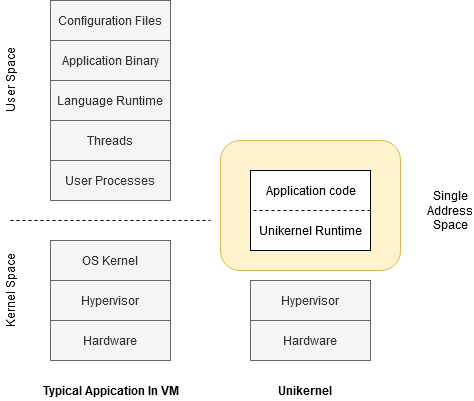
\includegraphics[width=\textwidth]{pictures/UnikernelDesign.png}
  \caption{Συμβατική εικονική μηχανή - \en{Unikernel}}
  \label{fig:genUnikernel}
\end{figure}

Δημιουργείται, συνεπώς, μια ταχύτατη, μικρή και εστιασμένη
εικονική μηχανή, η οποία μπορεί να εκτελεστεί αυτόνομα
επάνω σε ένα \en{hypervisor} ή στο ίδιο το υλικό, δίχως την
ανάγκη ενός υφιστάμενου λειτουργικού συστήματος. Η εκκίνηση
(\en{boot}) είναι ταχύτατη, τάξης μεγέθους ανώτερη από ένα
συμβατικό λειτουργικό στο οποίο εκτελείται αντίστοιχη
εφαρμογή. Ταυτόχρονα, η ασφάλεια είναι αυξημένη καθώς η
εφαρμογή τρέχει στο δικό της περιβάλλον, αποκομμένη από
την συνεκτέλεση άλλων στο ίδιο χώρο χρήστη, όπως ισχύει στα συμβατικά
λειτουργικά συστήματα. Τέλος, οι
ανάγκες σε πόρους ελαχιστοποιούνται, καθώς μπορεί να ανατεθούν
ακριβώς όσους χρειάζεται η συγκεκριμένη εφαρμογή,
ενώ σε ένα συμβατικό λειτουργικό θα έπρεπε να μεριμνήσει ο σχεδιαστής ώστε
να υπάρχουν διαθέσιμοι πόροι για όλες τις εφαρμογές που μπορεί
να εκτελεστούν παράλληλα, ακόμα και αν δεν εκτελούνται πράγματι.







%FRAMEWORKS
\subsection{\en{Frameworks}}

Ακολουθεί μια χρήσιμη αναφορά σε διάφορα \en{unikernel framework}
που υπάρχουν την στιγμή που γράφονται αυτές οι γραμμές,
καθώς και μια ανάλυση των χαρακτηριστικών του καθενός.

\subsubsection{\en{MirageOs}}

Το \en{MirageOs} αποτελεί ένα από τα παλαιότερα και πιο διαδεδομένα
\en{frameworks}. Το \en{MirageOs} δημιουργήθηκε στο εργαστήριο
υπολογιστών του πανεπιστημίου του \en{Cambridge}. Ο σκοπός των δημιουργών ήταν
να λύσουν το
πρόβλημα που προκύπτει κατά την εικονικοποίηση συστημάτων, πως
προστίθεται ένα επιπλέον στρώμα λογισμικού, οδηγώντας σε μη
βέλτιστη συμπεριφορά των εικονικών μηχανων\cite{riseOfVirtLibOS}. Μάλιστα στο
ίδιο εργαστήριο είχε αναπτυχθεί το 2003 ο \en{hypervisor Xen}\cite{xenArtofVirt}.
Ο σκοπός του \en{project}, είναι να ανακατασκευαστούν οι εικονικές
μηχανές, από το επίπεδο της εφαρμογής μέχρι και το επίπεδο
του πυρήνα ώστε να είναι καλύτερα αλληλοσυνδεδεμένα στην βάση
ενός \en{library operating system}.
\newline

Για την δημιουργία του \en{unikernel} με βάση το \en{MirageOS}
χρησιμοποιείτε η γλώσσα
\en{OCaml}, μια γλώσσα αρκετά υψηλού επιπέδου. Η επιλογή της
συγκεκριμένης γλώσσας έχει γίνει διότι αυτή επιτρέπει την
ανάπτυξη \en{type safe} εφαρμογών με μέλημα την προστασία της
μνήμης από \en{memory leaks}. Τέτοια σφάλματα σχετίζονται με
την μη ορθή χρήση των διαφόρων τύπων δεδομένων από μια γλώσσα.
Η \en{OCaml} για να το πετύχει αυτό διαθέτει στατικό έλεγχο των
τύπων (\en{static type check}), οπότε οι τυχόν ασυμφωνίες εντοπίζονται
κατά το \en{compile} και όχι κατά την εκτέλεση, καθώς και ένα
διακριτικό συλλέκτη σκουπιδιών (\en{garbage collector}), ο οποίος
ανακυκλώνει την αποδεσμευμένη μνήμη.
\newline

Για να αξιοποιηθούν καλύτερα τα νέα χαρακτηριστικά του \en{mirageOs},
αναπτύχθηκαν από την αρχή σημαντικά συστατικά ενός παραδοσιακού
λειτουργικού συστήματος, όπως το \en{network} και \en{storage stack}.
Έτσι, γράφτηκαν βιβλιοθήκες για \en{TCP/IP, ΗΤΤP, DNS} κ.α. στην
\en{Ocaml}. Το αποτέλεσμα είναι ένα ασφαλές και αρθρωτό \en{framework},
ιδανικό να υποστηρίξει \en{web υπηρεσίες}. Υπάρχουν διάφορα
παραδείγματα \en{self-hosted} διαδικτυακών ιστοσελίδων που εκτελούνται
ως \en{MirageOs} εφαρμογές επάνω σε κάποιον \en{hypervisor}, όπως το \en{Xen}\cite{overMirage}.
\newline

Ένα μειονέκτημα είναι πως η εκτελούμενη εφαρμογή πρέπει να
είναι γραμμένη σε \en{OCaml} για να μπορεί να εκτελεστεί με το
\en{MirageOs}. Αυτό συνήθως δεν ισχύει για τα περισσότερα
προγράμματα, με αποτέλεσμα να απαιτείται ανάπτυξη της εφαρμογής
από την αρχή. Τέλος, οι υποστηριζόμενες πλατφόρμες είναι το
\en{Xen}, και το \en{KVM} αν χρησιμοποιηθεί το \en{solo5 framework}, που
θα αναλυθεί στην συνέχεια.

\subsubsection{\en{IncludeOS}}

Το \en{IncludeOS} είναι ένα μινιμαλιστικό, ανοιχτού κώδικα, \en{unikernel}
\en{framework}, το οποίο στοχεύει σε εφαρμογές και υπηρεσίες
γραμμένες σε γλώσσα \en{C++}, και που στοχεύουν στο \en{cloud}. Πρόκειται
για ένα από τα νεότερα \en{unikernel frameworks}, και στοχεύει στην
ανάπτυξη τέτοιων εικονικών μηχανών με την ευκολία που έχει η
συμπερίληψη μια βιβλιοθήκης κατά την ανάπτυξη των εφαρμογών.
Γράφοντας απλά \en{\#include<os>}, κυριολεκτικά κατά το \en{linking} της
εφαρμογής μας θα συμπεριληφθεί ένα μικροσκοπικό λειτουργικό
σύστημα και θα παραχθεί μια πλήρης εικόνα εικονικής μηχανής\cite{includeOS}.
\newline

Σε αντίθεση με αρκετά άλλα \en{frameworks}, το\en{ IncludeOs} δεν έχει
κληρονομήσει από κάποιο άλλη πλατφόρμα αυτούσιες τις
βιβλιοθήκες ή και τα συστατικά στοιχεία που χρειάζονται οι εφαρμογές.
Αντίθετα όλα αυτά έχουν γραφτεί από την
αρχή σε \en{C++}, με έμφαση στα \en{unikernel} χαρακτηριστικά του.
Με αυτόν τον τρόπο έχει επιτευχθεί αποδοτική διαχείριση
των πόρων και των απαιτήσεων σε μνήμη, αποδοτική διαδικασία
\en{deployment}, και ανεξαρτησία από την πλατφόρμα εικονικοποίησης.
Αυτή την στιγμή τα \en{unikernel} που παράγονται από το
\en{IncludeOs} μπορούν να εκτελεστούν επάνω στους περισσότερους
δημοφιλείς επόπτες, καθώς και στο \en{openStack}\cite{Orestis}.
\newline

Το \en{IncludeOs} χαρακτηρίζεται από χαμηλό αποτύπωμα μνήμης,
υποστήριξη για \en{C++11/17}, τις κλασσικές βιβλιοθήκη \en{C++} κ.α..
Επίσης, υπάρχει υποστήριξη και για την βιβλιοθήκη της \en{C}
γλώσσας, δίνοντας μια συμβατότητα με κάποιες \en{POSIX} εφαρμογές\cite{includeOS}.
Τέλος, είναι αρκετά ενδιαφέρον το γεγονός πως υλοποιήθηκε από την αρχή
μια αρθρωτή στοίβα δικτύου εστιασμένη στο \en{project}, που
επιτρέπει ταχύτερη ανταλλαγή πακέτων και υψηλότερη απόδοση.
\newline

Μια εφαρμογή σε \en{IncludeOs}, δεν εκκινεί όπως μια παραδοσιακή
εφαρμογή για συμβατικό λειτουργικό με μια \en{main()}, αλλά με
την εντολή \en{Service::start}. Αυτό πρόκειται την υπηρεσία
(\en{service)} που οφείλει να υλοποιεί ο προγραμματιστής αν θέλει
να εκκινήσει η εφαρμογή του. Οι εφαρμογές πρέπει να γράφονται
υποχρεωτικά σε γλώσσα \en{C++}. Όπως και στα περισσότερα
\en{unikernel framework}, δεν υπάρχει υποστήριξη για εικονική
μνήμη ούτε ο διαχωρισμός μεταξύ \en{user space} και \en{kernel space}.
Τέλος, εφόσον απουσιάζουν τα νήματα και εκτελείται
κώδικας μόνο μιας διεργασίας, πολυνηματικές εφαρμογές ή εφαρμογές
που στηρίζονται στην παράλληλη εκτέλεση πολλών εργασιών
πρέπει να ξαναγραφούν ώστε να ταιριάζουν με τα
χαρακτηριστικά του \en{framework}\cite{Charalampos}.

\subsubsection{\en{OSv}}

Το \en{OSv} αποτελεί ένα σύγχρονο λειτουργικό σύστημα το οποίο
εστιάζει στην εκτέλεση των εφαρμογών στο \en{cloud}.
Δημιουργήθηκε το 2013 από την \en{Cloudious Systems} με σκοπό
να τρέχει επάνω σε μια πληθώρα από \en{hypervisors}, και να
υποστηρίζει τις περισσοτερες από τις δημοφιλείς γλώσσες,
\en{C, C++, Java, Ruby, NodeJS} κλπ. Πρόκειται, συνεπώς, για
ένα \en{unikernel framework} ικανό να εκτελέσει  \en{single-process linux}
εφαρμογές\cite{Orestis}.
\newline

Σε σχέση με τα υπόλοιπα \en{unikernel frameworks}, το \en{OSv}
χαρακτηρίζεται ως ένα λειτουργικού γενικού σκοπού, που
μπορεί να μετατρέψει σχεδόν κάθε εφαρμογή σε \en{unikernel}.
Ταυτόχρονα, υποστηρίζει τους περισσότερους γνωστούς
επόπτες, όπως \en{Xen, KVM, QEMU, VMware, GCE}. Αυτή η ιδιότητα το
υποχρεώνει να είναι ένα από το πιο σύνθετα, και συνεπώς
μεγάλα σε μέγεθος, \en{unikernel}, όπου η παραγόμενη εικονική
μηχανή είναι τάξης μερικών δεκάδων \en{megabytes}. Εν συγκρίσει, τα περισσότερα
\en{unikernels} εμφανίζουν συνηθισμένο μέγεθος μερικών \en{kilobytes}\cite{Orestis}.
\newline

Όπως και στα περισσότερα \en{unikernel} περιβάλλοντα, υπάρχει
μόνο μια εκτελούμενη διεργασία ανά πάσα στιγμή και
απουσιάζει ο διαχωρισμός \en{user space} και \en{kernel space},
οπότε όλος ο κώδικας τρέχει σε ένα μοναδικό χώρο μνήμης.
Αυτό προφανώς οδηγεί στην μείωση της καθυστέρησης της
εκτέλεσης που σχετίζεται με την αλλαγή του \en{context}.
\newline

Ένα αξιοσημείωτο χαρακτηριστικό του είναι η χρήση
χρονοδρομολογητή (\en{scheduler}) για τον συγχρονισμό
των εικονικών επεξεργαστών (\en{virtual CPUs}), χωρίς την
χρήση \en{spinlocks}. Tα \en{spinlocks} χρησιμοποιούνται όταν
τα νήματα που πρέπει να συγχρονιστούν ως προς την
πρόσβαση σε ένα κοινόχρηστο πόρο, όπως π.χ. μια ευαίσθητη
περιοχή μνήμης, δεν μπορούν να κοιμηθούν. Στα
εικονικοποιημένα περιβάλλοντα είναι όμως πιθανόν
μια εικονική \en{CPU} να πάψει προσωρινά να εκτελεί
εντολές, με αποτέλεσμα να υποχρεώνει τις υπόλοιπες
να αναμένουν άεργες σπαταλώντας πόρους. Επιλέχθηκε,
συνεπώς, όλα τα νήματα στο \en{OSv}, εκτός από τον ίδιο τον \en{scheduler},
να είναι σε θέση να κοιμηθούν, και άρα να μην απαιτούνται
\en{spinlocks}\cite{OSV-optimizing}. Επίσης, δεδομένου πως η εκτέλεση διαδικτυακών
εφαρμογών στο \en{cloud} θα είναι ο κύριος στόχος τέτοιων \en{frameworks},
οι συσκευές δικτύου σχεδιάστηκαν από την αρχή. Με την
τεχνική που ονομάζεται κανάλια δικτύου (\en{network channels}),
τα πακέτα που έρχονται με διακοπές από το δίκτυο
επεξεργάζονται και ταξινομούνται σε ξεχωριστά νήματα,
μέσα στο ίδιο \en{context} με την εκτελούμενη εφαρμογή
επιτυγχάνοντας αυξημένη επίδοση ταχύτητα, απλοποιώντας
τον ανταγωνισμό για τους μηχανισμούς από τα διάφορα περιβάλλοντα επικοινωνίας
που χρησιμοποιούν το δίκτυο. Τέλος, πολύ ενδιαφέρον είναι
πως, σε αντίθεση με τα αρκετά άλλα \en{unikernel frameworks},
στο \en{OSv} υπάρχει υποστήριξη για εικονική μνήμη. Έτσι
εφαρμογές που στηρίζονται σε αυτή, π.χ. με χρήση της
\en{mmap()}, μπορούν να μετατραπούν πιο εύκολα σε \en{unikernel}\cite{OSV-optimizing}.

\subsubsection{\en{Solo5}}

Το \en{Solo5} δεν πρόκειται για ένα πλήρες \en{unikernel framework}, όπως
τα υπόλοιπα που αναφέρονται στην παρούσα εργασία, αλλά ένα ενδιάμεσο
στρώμα επάνω στο οποίο μπορεί να αναπτυχθεί ένα \en{unikernel}.
Ξεκίνησε από τον \en{Dan Williams} της \en{IBM Research}, με σκοπο να
επιτρέψει στο \en{MirageOs} να εκτελείται επάνω στον επόπτη \en{linux-KVM}.
Πλέον έχει εξελιχθεί σε ένα \en{sandbox} περιβάλλον εκτέλεσης και
απομόνωσης επάνω στο οποίο μπορεί να εκτελεστεί ένα μεγάλος
αριθμός από \en{Unikernel} ή γενικότερα από \en{library operating systems}.
Μπορούμε να το φανταστούμε ως ένα στρώμα λογισμικού, το οποίο
κάθεται ανάμεσα στον επόπτη και στο \en{Unikernel}\cite{solo5}.
\newline

Όπως έχει αναφερθεί, βασικό συστατικό της φιλοσοφία των \en{Unikernel},
και γενικώς των \en{library operating systems}, είναι η αφαίρεση
των περιττών συστατικών που υπάρχουν σε ένα συμβατικό
λειτουργικό. Το \en{Solo5} πηγαίνει αυτή την ιδέα ένα βήμα παραπέρα,
θεωρόντας τώρα όλο το \en{unikernel} ως μια διεργασία της οποίας
η διεπαφή με το \en{hypervisor} ή και γενικά με όλο το λειτουργικό
σύστημα επανασχεδιάζεται. Αρχικά, είναι επιθυμητό η διεπαφή να είναι
\en{lightweight} και όσο πιο δυνατόν \en{legacy-free}. Για παράδειγμα
το \en{QEMU}, ένα από τα πιο δημοφιλή \en{hypervisors}, εκθέτει
στο \en{unikernel} μια πληθώρα από εικονικές συσκευές, άχρηστες
για το \en{unikernel}, ακριβώς επειδή το \en{QEMU} είναι σχεδιασμένο
να υποστηρίζει πλήρη λειτουργικά συστήματα και όχι αποκλειστικά
\en{unikernel}\cite{solo5Monitor}. Το \en{Solo5} περιορίζει την διεπαφή μόνο στα
συστατικά που χρειάζεται το \en{unikernel}. Το κέρδος είναι πως με την
αυξημένη αφαίρεση μπορούμε να πετύχουμε μεγαλύτερη φορητότητα
(\en{portability}) των \en{unikernel} ανάμεσα σε διάφορες πλατφόρμες\cite{Orestis}.
Είναι εμφανής η αναλογία των σχέσεων μεταξύ διεργασίας-λειτουργικού
και \en{unikernel-hypervisor}.
\newline

Επιπροσθέτως, το \en{Solo5} εισάγει την έννοια του προγράμματος
φύλακα (\en{tender}), το οποίο ονομάζει \en{hvt (harware virtualized tender)}.
Ο φύλακας είναι ένα εξειδικευμένα στρώμα διεπαφής για \en{unikernels}.
Ο ρόλος του μοιάζει με αυτόν που έχει παραδοσιακά το \en{QEMU}, όμως
όπως αναφέρθηκε, το \en{QEMU} είναι γενικού σκοπού, ενώ ο \en{hvt}
στοχεύει σε ένα συγκεκριμένο \en{unikernel}. Το \en{interface}, λοιπόν,
που ‘βλέπει’ το \en{unikernel} είναι αυτό ακριβώς που έχει το ίδιο
ανάγκη, και τίποτα παραπάνω, μειώνοντας έτσι την επιφάνεια
επίθεσης και το ενδεχόμενο κάτι να δυσλειτουργήσει.
\newline

Το κέρδος αυτής της μείωσης της επιφάνειας του \en{interface}, είναι
πολύ σημαντικό. Η μη ανάγκη για αρχικοποίηση των περιττών
στοιχείων επιτρέπει στα \en{unikernel} να εκκινούν (\en{boot}) αισθητά
πιο γρήγορα από άλλα. Η ασφάλεια βρίσκεται σε υψηλότερα επίπεδα,
καθώς δεν υπάρχουν περιττά \en{components}, με τα οποία θα μπορούσε
κάποιος να επηρεάσει το \en{unikernel}. Τέλος, το σύνολο \en{unikernel-monitor},
μειώνεται δραματικά σε μέγεθος, καθώς δεν χρειάζεται η παρουσία
ενός \en{general-purposed} και ‘βαριού’ \en{monitor} όπως το \en{QEMU}, αλλά ένα
\en{lightweight} και γρήγορου\cite{solo5Monitor}\cite{Orestis}.
\newline

\begin{figure}[h]
  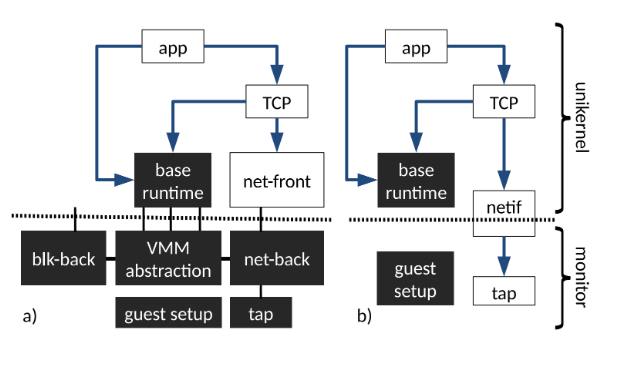
\includegraphics[width=\textwidth]{pictures/unikern-unikernel+monitor(solo5).PNG}
  \caption{\en{a. Monitor} γενικού σκοπού \en{b. Monitor} ειδικού σκοπού}
  \label{fig:solo5}
\end{figure}


Το \en{Solo5} χρησιμοποιείται κυρίως από το \en{MirageOS}, που ήταν και ο
αρχικός στόχος του, και από το \en{IncludeOS}. Επίσης υποστηριζόμενες
πλατφόρμες-\en{hypervisors} είναι \en{linux-KVM, FreeBSD-VMM} ως \en{hvt},
και γενικά οποιοσδήποτε \en{hypervisor} σε \en{x}86 αρχιτεκτονική αρκεί
να υποστηρίζει με την σειρά του \en{virtio} συσκευές, όπως \en{QEMU/KVM}\cite{Orestis}.
Σημειώνεται επίσης, πως το \en{solo5 } ούτε στοχεύει ούτε υποστηρίζει την
απευθείας εκτέλεση στο υλικό (\en{bare-metal}).

\subsubsection{\en{Rumprun}}

Το \en{Rumprun} αποτελεί ένα \en{unikernel framework}, που έχει στηριχθεί
επάνω στα \en{rump kernels} και στοχεύει στην εκτέλεση οποιαδήποτε
\en{single-process POSIX} εφαρμογής. Αυτή είναι και η ιδέα που ώθησε
την δημιουργία του, δηλαδή να μπορεί να μετατραπεί οποιαδήποτε
\en{POSIX} εφαρμογή σε \en{unikernel}, με όσο τον δυνατόν ελάχιστες αλλαγές
στον κώδικά της\cite{Orestis}\cite{RumprunXen}.
\newline

Το \en{project} των \en{rump kernels} αποτελεί εγχείρημα ώστε να προσφέρονται
αυτούσιοι οι \en{drivers} και τα συστατικά στοιχεία ενός λειτουργικού
συστήματος, ώστε να επιτρέπεται η ανάπτυξη ελαφρών, αρθρωτών και
ασφαλών εικονικών μηχανών. Τα \en{rump kernels}, χρησιμοποιούν τους
\en{drivers} του \en{NetBSD} λειτουργικού συστήματος, το οποίο με την σειρά του
έχει σχεδιαστεί ώστε να είναι όσο το δυνατόν \en{modular}, με αποτέλεσμα
οι \en{drivers} του να είναι αρκετά φορητοί και ανεξάρτητοι πλατφόρμας\cite{noOSnoProb}.
\newline

Μια δεύτερη ιδέα που οδήγησε στο \en{Rumprun}, είναι αυτή του \en{anykernel}.
Παραδοσιακά, τα λειτουργικά συστήματα χαρακτηρίζοντας από την
αρχιτεκτονική του μονολιθικού πυρήνα (\en{monolithic kernel}), στην
οποία όλες οι προνομιούχες ενέργειες, όπως η χρονοδρομολόγηση, η
διαχείριση της εικονικής μνήμής, οι εκτέλεση των οδηγών των συσκευών,
γίνονταν στον χώρο του πυρήνα με αυξημένα προνόμια. Όσο μεγάλωνει
η πολυπλοκότητα των συστημάτων, αυτή η προσέγγιση γίνεται όλο και
πιο δυσκίνητη και ανελαστική. Σε απάντηση αυτού του προβλήματος,
εμφανίζονται άλλες εναλλακτικές όπως τα \en{hybrid kernels} κ.α. Μια
από αυτές είναι το \en{anykernel}, όπου περιγράφεται ένας κώδικας βάσης
από τον οποίο μπορούν να εξαχθούν από τον πυρήνα οι \en{drivers} και να
 εκτελεστούν με μικρή ή και καθόλου τροποποίηση σε διαφορετικό
 περιβάλλον ή ακόμα και στον χώρο χρήστη. Αυτός ο διαχωρισμός μεταξύ των
 \en{drivers} και πιο αυξημένης σημασίας στοιχείων του λειτουργικού δίνει μεγαλύτερη
 ευελιξία στο όλο σύστημα\cite{noOSnoProb}\cite{interviewKantee}.
\newline

Αυτήν την στιγμή, τα \en{unikernel} από το \en{Rumprun} μπορούν να εκτελεστούν
επάνω στο \en{Xen}, στο \en{QEMU/KVM}, αλλά και απευθείας επάνω στο υλικό (\en{bare metal}).
\newline

Για την υλοποίηση της παρούσας εργασίας επιλέγουμε το \en{Rumprun} ως
\en{unikernel framework}, επάνω στο οποίο εργαζόμαστε, οπότε οφείλουμε να το
αναλύσουμε διεξοδικά στην συνέχεια.
\newline

Αυτά ήταν κάποια από τα πιο γνωστά και σημαντικά \en{unikernel frameworks}.
Υπάρχουν πολλά ακόμα όπως το \en{ClickOS, Clive, LING, RuntimeJS, Nanos} κ.α\cite{wikiUnikernel}.




%Rumprun
\subsection{\en{Rumprun}}

\subsubsection{Ιστορία}

Οι \en{rump kernels} και το \en{Rumprun} γεννήθηκαν αρχικά από την ανάγκη
εκτέλεσης \en{driver}, και συγκεκριμένα του συστήματος αρχείων (\en{file systems}),
του \en{NetBSD} σε χώρο χρήστη. Παρατηρήθηκε πως είναι πολύ πιο γρήγορο
και αποτελεσματικο να αναπτύσσονται \en{drivers} με αυτόν τον τρόπο,
παρά σε ένα εικονικοποιμένο περιβάλλον όπως ήταν το σύνηθες. Με την
πάροδο του χρόνου, οι \en{drivers} γράφονταν ώστε να είναι όλο και
πιο ανεξάρτητοι της πλατφόρμας και φορητοί, έτσι προέκυψαν οι
\en{rump kernels}. Εν τέλει, προσφέρθηκε η δυνατότητα να εκτελούνται αυτοι
οι \en{drivers} επάνω στον \en{Xen hypervisor}, το οποίο με την σειρά του
γέννησε το \en{Rumprun}\cite{RumprunXen}\cite{interviewKantee}.
\newline

Όπως αναφέρθηκε, το \en{Rumprun framework} στηρίζεται στην ιδέα του
\en{anykernel}, την οποία έννοια επινόησε ο \en{Antii Kantee}\cite{interviewKantee}, δημιουργός
των \en{rump kernels} και του \en{Rumprun}. Τα περισσότερα συμβατικά λειτουργικά συστήματα
στηρίζονται στην μονολιθική (\en{monolithic}) αρχιτεκτονική, όπου όλες
οι ενέργειες, οι οποίες απαιτούν αυξημένη δικαιοδοσία, όπως η διαχείριση
μνήμης, ο \en{scheduler}, το σύστημα αρχείων αλλά και οι \en{drivers} για
τις περιφερειακές συσκευές, εκτελούνται μέσα στον χώρο πυρήνα.
Από τη μία αυτό προσφέρει ασφάλεια, από την άλλη, όμως, δυσκολεύει
την ανάπτυξη των συστατικών (\en{components}) και ειδικά των \en{drivers}.
\newline

Σε απάντηση του παραπάνω προβλήματος,έχουν εμφανιστεί διαφορετικές
αρχιτεκτονικές λειτουργικών, όπως οι \en{microkernels, exokernels} κ.α..
Κύριο χαρακτηριστικό αυτών είναι ότι οι πολύ σημαντικές
δραστηριότητες του πυρήνα, όπως η διαχείριση μνήμης και ο
\en{scheduler}, παραμένουν στο χώρο του πυρήνα, ενώ λιγότερο σημαντικά
συστατικά, όπως οι \en{drivers} των συσκευών και το σύστημα αρχείων,
εκτελούνται στον χώρο χρήστη. Αυτό προσφέρει μεγαλύτερη ευελιξία
και ασφάλεια κατά την ανάπτυξη των τελευταίων συστατικών.
\newline

\begin{figure}[h]
  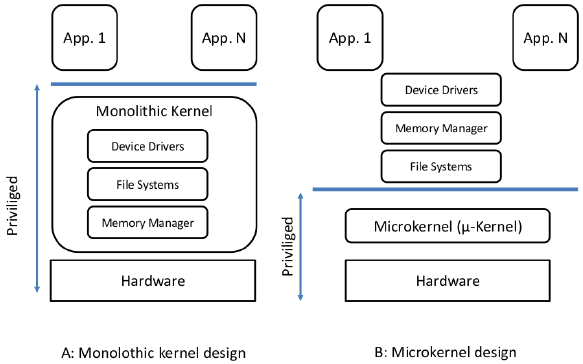
\includegraphics[width=\textwidth]{pictures/mono-micro_kernels.png}
  \caption{Α.Μονολιθική και \en{Microkernel} αρχιτεκτονική πυρήνα}
  \label{fig:microkernels}
\end{figure}

Το σκεπτικό πίσω από τον όρο \en{anykernel} επεκτείνει περαιτέρω τον ανώτερο διαχωρισμό
των λειτουριών ενός συστήματος που παραδοσιακά επιτελούνται εντός του πυρηνα.
Πλέον, οι \en{drivers} του συστήματος
ανεξαρτητοποιούνται από το σύστημα στο οποίο εν τέλει θα
εκτελεστούν. Αναφερόμαστε σε μια αρχιτεκτονικά αγνωστική
προσέγγιση, όπου οι \en{drivers} μπορούν είτε να ενσωματώνονται
σε κάποιο μονολιθικό πυρήνα, σε κάποιο \en{microkernel}, σε
κάποιο \en{exokernel}, γενικά σε πυρήνες διαφορετικών αρχιτεκτονικών,
ή να εκτελούνται ως διεργασία στο \en{user space} χωρίς κάποια
αλλαγή στον κώδικά τους. Ως \en{drivers} δεν εννοούμε μόνο τους
οδηγούς συσκευών, αλλά και το σύστημα αρχείων, την στοίβα
δικτύου κ.α.. Υπάρχει, λοιπόν, μια εγγενής φορητότητα των
\en{drivers}\cite{noOSnoProb}. Το λειτουργικό σύστημα \en{NetBSD} ταιριάζει στον
ορισμό του \en{anykernel}\cite{interviewKantee}.
\newline

Σχετική έννοια είναι αυτή των \en{rump kernels}. Με τον όρο \en{rump }
εννοούμε ένα κατάλοιπο ενός μεγαλύτερου αρχικού συνόλου.
\en{Rump kernel}, λοιπόν, είναι ένα εικονικοποιημένο στιγμιότυπο
ενός συνόλου από \en{drivers}, οι οποίοι τρέχουν εκτός του
μονολιθικού πυρήνα. Αυτό πρακτικά μεταφράζεται σε έναν
πυρήνα ενός παραδοσιακού λειτουργικού συστήματος, από
το οποίο έχουν αφαιρεθεί διάφορα κομμάτια, όπως η εικονική
μνήμη και ο συγχρονισμός μεταξύ διεργασιών. Το υπόλειμμα
(\en{rump}) είναι οι \en{drivers} και οι απολύτως απαραίτητες ρουτίνες, ώστε
να μπορεί να εκτελεστεί μία διεργασία\cite{Orestis}. Μπορούμε να φανταστούμε
τους \en{rump kernels} σαν πυρήνας-ως-υπηρεσία (\en{kernel-as-a-service}).
Οι \en{rump kernels} που δημιουργήθηκαν από τον \en{Antii Kantee}
εξάγουν τους \en{drivers} και τα στοιχεία από το λειτουργικό σύστημα
\en{NetBSD}, δηλαδή από τον \en{open-source} πηγαίο κώδικά του\cite{interviewKantee}.
\newline

Το \en{rumprum unikernel} είναι μια εφαρμογή των \en{rump kernels}, που
έχει στόχο να εκτελούνται προγράμματα ως \en{unikernel}. Υπενθυμίζεται
ότι ο αρχικός στόχος του εγχειρήματος των \en{rump kernel} ήταν
να εκτελούνται αυτόνομα \en{drivers} στο \en{user space}, ώστε να
διευκολύνεται η ανάπτυξη και η αποσφαλμάτωσή του. Όμως, με
την πάροδο του χρόνου, αποδείχθηκε πως οι \en{rump kernels} μπορούν
να εκτελεστούν ως εικονικοποιημένος \en{guests} επάνω στον \en{Xen hypervisor}.
Η πρώτη εφαρμογή αυτού του «παντρέματος» ήταν η εκτέλεση ελαφρών
\en{router} ή \en{firewalls} ως \en{guests}, λειτουργίες που παραδοσιακά
βρίσκονταν στον χώρο ενός μονολιθικού πυρήνα. Σύντομα προστέθηκε
και η ύπαρξη μια διεπαφής από τον χώρο χρήστη, δηλαδή ένας
τρόπος να καλούνται οι κλήσεις συστήματος\cite{RumprunXen}. Με όλα αυτά τα
επίπεδα λογισμικού διαθέσιμα, είναι προφανές ότι οι \en{rump kernels}
έχουν την δυνατότητα να παράγουν \en{unikernels}, τα οποία ονομάστηκαν
\en{Rumprun unikernels}. Η σχέση μεταξύ του \en{Rumprun} και των \en{rump kernels},
είναι πως για την ανάπτυξη του \en{unikernels}, το \en{Rumprun} επιλέγει
από το σύνολο που προσφέρουν οι \en{rump kernels} μόνο τα στοιχεία
που είναι απαραίτητα για την εκτέλεση μιας συγκεκριμένης εφαρμογής,
το οποίο σημαίνει πως το \en{Rumprun} είναι μια από τις πολλές
εφαρμογές (\en{use cases}) των \en{rump kernels}. Η εικόνα \ref{fig:any_rumpk_Rumprun}
παρουσιάζει καλύτερα την σχέση μεταξύ του \en{anykernel} των \en{rump kernels}
και του \en{Rumprun unikernel}.
\newline

\begin{figure}[h]
  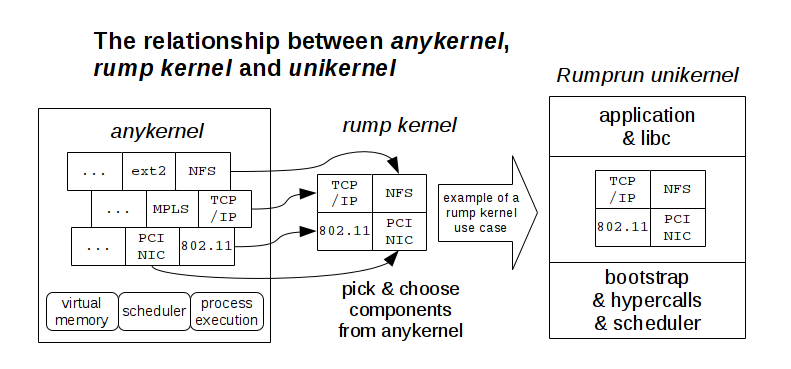
\includegraphics[width=\textwidth]{pictures/anykernel-rumpkernel.PNG}
  \caption{Σχέση μεταξύ \en{anykernel-rump kernels-Rumprun}}
  \label{fig:any_rumpk_Rumprun}
\end{figure}


\subsubsection{Δομή και Ανάπτυξη του \en{Unikernel}}

Η στοίβα λογισμικού του \en{Rumprun}, θυμίζει σε ένα βαθμό την στοίβα
εκτέλεσης μιας διεργασίας σε κάποιο συμβατικό λειτουργικό
σύστημα. Στο ανώτερο επίπεδο βρίσκεται ο κώδικας της εφαρμογής,
ο οποίος στηρίζεται σε βιβλιοθήκες του \en{user space}, όπως π.χ. η \en{libc}
για την γλώσσα \en{C}. Από κάτω βρίσκονται οι κώδικας που αναλαμβάνει
να καλέσεις τις κλήσεις συστήματος (\en{system calls}) προς τον
πυρήνα. Μια διαφορά που υπάρχει στο \en{Rumprun} είναι πως οι κλήσεις
αυτές δεν γίνονται με
κάποια \en{trap} εντολή ώστε να αλλάξει το επίπεδο προνομίων με το
οποίο εκτελείται ο κώδικας, αλλα καλείται απλά μια απλή συνάρτηση
βιβλιοθήκης η οποία αναλαμβάνει να εξυπηρετήσει την αίτηση.
Υπενθυμίζεται πως σε \en{unikernel} όλη η εκτέλεση γίνεται σε ένα
μοναδικό ενιαίο χώρο μνήμης, δεν υπάρχει διάκριση μεταξύ
\en{user space} και \en{kernel space}. Για να το πετύχει αυτό, το
\en{Rumprun} αντικαθιστά όλες τις κλήσεις συστήματος (\en{system calls})
του \en{NetBSD} δικές του κλήσεις πυρήνα (\en{rump kernel calls}), οι
οποίες είναι στην ουσία κλήσεις συναρτήσεων (\en{library calls}).
Από αυτό το επίπεδο και μέχρι το επίπεδο του επόπτη βρίσκεται
ό,τι θα έπρεπε να βρίσκεται στον πυρήνα ενός συμβατικού λειτουργικού.
\newline

Εύλογα θα περίμενε κανείς, στα κατώτερα επίπεδα να βρίσκονται
κομμάτια λογισμικού μόνο από τους \en{rump kernels}. Εντούτοις,
οι \en{rump kernels} δεν σχεδιάστηκαν ώστε να τρέχουν επάνω σε κάποιο
επόπτη ως εικονική μηχανή, οπότε τους λείπει η δυνατότητα να
επικοινωνούν με το χαμηλότερο επίπεδο του επόπτη. Ταυτόχρονα
απουσιάζουν και οι μέθοδοι εκκίνησης (\en{bootstrap}), χρονοδρομολόγησης,
διακοπές (\en{interrupt}), και διαχείριση των σελίδων της μνήμης.
Για αυτόν ακριβώς τον λόγο, στον στοίβα του \en{Rumprun} κάτω
από το κομμάτι των \en{rump kernels} έχει προστεθεί ένα στρώμα
υλικού που ονομάζεται \en{Bare Metal Kernel (bmk)}, και που
ρόλος του είναι να επιτελεί όλες αυτές τις σημαντικότατες
ανώτερες λειτουργίες.
Ο \en{bmk} αποτελείται τόσο από κώδικα
που είναι κοινός για κάθε πλατφόρμα στην οποία στοχεύει το
\en{Rumprun}, όσο και από κώδικα ειδικό για κάθε πλατφόρμα
ξεχωριστά\cite{Orestis}. Παράλληλα, υπάρχει και ένας μηχανισμός
επικοινωνίας των \en{rump kernels} με τον \en{bmk}, που ονομάζεται
\en{rumpuser}\cite{noOSnoProb}. Οι βασικοί στόχοι του \en{Rumprun} είναι είτε ο \en{Xen hypervisor},
είτε το \en{KVM} των \en{Linux}, είτε απευθείας το υλικό (\en{bare metal}).
\newline

Η δομή της στοίβας φαίνεται στην εικόνα \ref{fig:RumprunStack}
\newline
\begin{figure}[h]
  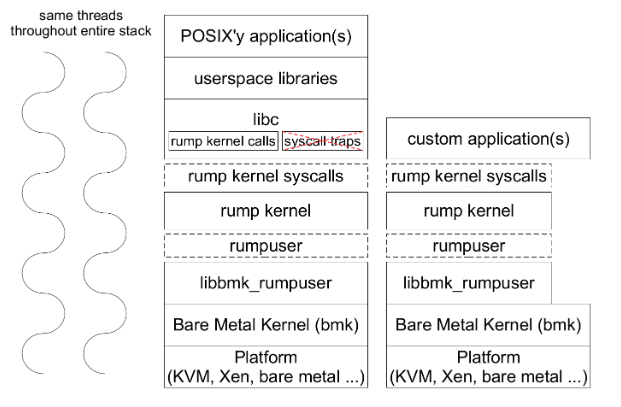
\includegraphics[width=\textwidth]{pictures/rumprun-stack.PNG}
  \caption{Στοίβα λογισμικού \en{rump kernels/Rumprun}}
  \label{fig:RumprunStack}
\end{figure}


Αξίζει, επίσης, να περιγραφεί η διαδικασία ανάπτυξης ενός \en{unikernel} με
το \en{Rumprun framework}. Η διαδικασία αποτελείται χονδρικώς από τέσσερα βήματα.
\begin{enumerate}
  \item Αρχικά αναπτύσσεται ο κώδικας της εφαρμογής σε
  \en{userspace}. Το \en{Rumprun} στοχεύει στην εκτέλεση \en{POSIX }
  εφαρμογές, οπότε η ανάπτυξη δεν διαφέρει από συμβατικά
  λειτουργικά, και συνήθως μπορεί να χρησιμοποιηθεί κώδικας
  από εφαρμογές ήδη γραμμένες για κάποια άλλη πλατφόρμα,
  όπως το \en{linux}. Ωστόσο, συγκεκριμένες λειτουργίες, όπως οι
  πολλές διεργασίες και η εικονική μνήμη δεν υποστηρίζονται,
  άρα εφαρμογές που στηρίζονται σε κλήσεις όπως \en{fork()} ή
  η \en{mmap()} πρέπει να προσαρμόζονται.

  \item Στην συνέχεια ο κώδικας γίνεται \en{compiled} σε
  ένα ή περισσότερα \en{object file}, όπως κατά συμβατικές
  διαδικασίες μεταγλώττισης. Το \en{Rumprun} στηρίζεται σε
  \en{cross-compilation}, όποτε δεν υπάρχει ανάγκη ύπαρξης
  κάποιου \en{unikernel} το οποίο μπορεί να μεταγλωτίζει, αλλά
  αντί αυτού προσφέρονται έτοιμοι \en{compilers}.

  \item Έπειτα έρχεται η σειρά του \en{linking} αυτών των
  αντικειμένων. Δεν πρόκειται για συμβατικό \en{linking},
  αλλά για \en{pseudo-linking}, καθώς οι εξαρτήσεις από το
  λειτουργικό σύστημα, για παράδειγμα οι κλήσεις συστήματος,
  δεν γίνονται \en{resolve} αλλά γίνεται μόνο έλεγχος για την
  ορθή συντακτική χρήση τους. Δεν επιτελείται, συνεπώς,
  κάποια σύνδεση με τα συστατικά του λειτουργικού συστήματος,
  που σε άλλη περίπτωση θα επέτρεπαν την επικοινωνίας κατά το
  \en{runtime}. Σε αυτή την φάση, παράγεται ένα αρχείο το οποίο
  θυμίζει εκτελέσιμο, όμως δεν είναι.

  \item Τέλος, επέρχεται το λεγόμενο \en{bake}, δηλαδή οι
  προαναφερθείσες εξαρτήσεις συνδέονται με τις συναρτήσεις
  των \en{rump kernels} που αναλαμβάνουν τις λειτουργίες που
  ζητούνται. Από το σύνολο των \en{drivers} των \en{rump kernels} εξάγονται
  μόνο όσοι χρειάζονται πραγματικά από την εφαρμογή. Ταυτόχρονα,
  προστίθεται και τα κομμάτια που χρειάζονται για την επικοινωνία
  με τον επόπτη στον οποίο στοχεύουμε.
\end{enumerate}
Με αυτόν τον τρόπο παράγεται το τελικό \en{unikernel}, η μικρή, ασφαλής
και γρήγορη εικονική μηχανή, που θα επιτελεί την λειτουργία για την
οποία σχεδιάστηκε.

\subsubsection{Γιατί \en{Rumprun}}

Όπως αναφέρθηκε, επιλέγεται το \en{Rumprun} να είναι το \en{framework}
επάνω στο οποίο εργαζόμαστε για την υλοποίηση της παρούσας
εργασίας. Θυμίζεται πως επιθυμείται να ενσωματώθει η λειτουργία
ελαστικής μνήμης \en{utmem}, η οποία αναλύεται αναλυτικότερα στην
συνέχεια, σε κάποιο \en{unikernel framework}. Το \en{rump kernels - Rumprun}
επιλέχθηκε ως κατάλληλο εργαλείο για τους εξής λόγους:

\begin{itemize}
  \item Ο μηχανισμός \en{utmem}, τουλάχιστον για το \en{frontend }
  που χρειάζεται να υλοποιηθεί από την αρχή, είναι ουσιαστικά ένας \en{driver}
  που επικοινωνεί με τον \en{hypervisor}. Αφού, λοιπόν, τα \en{rump kernels }
  επιτρέπουν την εξαγωγή \en{drivers} γραμμένους για το \en{NetBSD}, ένα
  \en{well-documented} λειτουργικό σύστημα, είναι εύλογο να ταιριάζουν
  στο \en{use case} μας και να διευκολύνουν το έργο μας.

  \item Το \en{Rumprun} στοχεύει στο να υποστηρίζει την
  μετατροπή των περισσότερων εφαρμογών οι οποίες υπακούν στο
   \en{POSIX} πρότυπο σε \en{unikernel}. Συνέπεια αυτού είναι πως δεν
   χρειάζεται ιδιαίτερη προσαρμογή επιλογών για να αναπτυχθεί \en{user space}
   κώδικα που να χρησιμοποιεί την \en{utmem}, καθώς η συντριπτική πλειοψηφία των
   προγραμματιστών γνωρίζει το \en{POSIX} πρότυπο,

  \item Στην στοίβα του \en{Rumprun} απουσιάζει από
  επιλογή των σχεδιαστών η εικονική μνήμη. Αυτή η επιλογή
  έγινε για να είναι όσο το δυνατόν ελαφρύτερα και απλούστερα
  τα τελικά \en{unikernel}. Ως εκ τούτου, το να ενσωματωθεί ο
  μηχανισμός της \en{utmem} σε ένα τέτοιο \en{unikernel framework},
  στην πράξη προσφέρει λύση σε ένα υπαρκτό ενδεχόμενο,
  δηλαδή στην διαχείριση περιορισμένης μνήμης. Η συγκεκριμένη εργασία
  επικεντρώνεται στην αντιμετώπιση αυτού του προβλήματος. Όπως θα
  φανεί και στην συνέχεια, πράγματι έχει ουσιαστική αξία η
  υλοποίηση της εργασίας.

\end{itemize}







\section{Μνήμη - \en{utmem}}

\subsection{Ιστορία}

Η διαχείριση της μνήμης ενός υπολογιστικού συστήματος είναι ένα
πολύ σημαντικό πρόβλημα που καλείται να λύσει o μηχανικός
υπολογιστικών συστημάτων. Η μνήμη αποτελεί σημαντικότατο πόρο, αν όχι τον σημαντικότερο.
Στα συμβατικά λειτουργικά συστήματα, κάθε διεργασία που εκτελείται
νομίζει πως βρίσκεται σε ένα ενιαίο χώρο μνήμης, τον οποίον
δεν μοιράζεται με άλλες εργασίες, οι οποίες μπορεί να βρίσκονται
στο σύστημα την στιγμή της εκτέλεσης. Το λειτουργικό σύστημα
από την άλλη, οφείλει να αντιστοιχεί αυτόν τον χώρο διευθύνσεων
που «βλέπει» η διεργασία (\en{virtual address space}), σε κάποιο κομμάτι της
φυσικής μνήμης του συστήματος (\en{physical address space}),
χρησιμοποιώντας μηχανισμούς και πολιτικές τόσο σε επίπεδο υλικού όσο και λογισμικού.
\newline

Πρόβλημα εμφανίζεται όταν η φυσική μνήμη του συστήματος γεμίσει
από εγγραφές και πλέον το λειτουργικό αδυνατεί να κατανείμει
περισσότερη στα προγράμματα. Αν δεν αντιμετωπιστεί αυτό το
πρόβλημα, και απλά αρνηθεί το λειτουργικό σύστημα να δώσει νέα
μνήμη, τότε προκύπτει ένα ασταθές, δυσλειτουργικό και
αναποτελεσματικό σύστημα. Η λύση, που πλέον ενσωματώνεται σε όλα
τα σύγχρονα λειτουργικά συστήματα όπως \en{Linux, Windows} κλπ, είναι
η ύπαρξη της εικονικής μνήμης (\en{virtual memory}), δηλαδή ενός
μηχανισμού που επιτρέπει στο σύστημα να δίνει στα προγράμματα την ψευδαίσθηση
πως υπάρχει περισσότερη διαθέσιμη μνήμη από την φυσική. Όταν η
μνήμη γεμίσει, σελίδες (\en{memory pages}) αυτής εναλλάσσονται (\en{swapping})
σε κάποιο άλλο αποθηκευτικό μέσο, διαθέσιμο στο σύστημα, το οποίο
συνήθως είναι κάποιος δίσκος. Όταν χρειαστεί να προσπελαστούν οι
σελίδες που έχουν μεταφερθεί στον δίσκο τότε αντιγράφονται πίσω
στην κύρια μνήμη, στην θέση κάποιων άλλων οι οποίες με την σειρά
του θα μετακινηθούν στον δίσκο. Οι αποθηκευτικοί δίσκοι έχουν
χωρητικότητα αρκετές φορές μεγαλύτερη από της φυσικής μνήμης,
έτσι λοιπόν επιτυγχάνεται η ψευδαίσθηση της περισσότερης
διαθέσιμης μνήμης\cite{wikiVirtMemory}. Το μεγάλο μειονέκτημα αυτής της τεχνικής
είναι πως, επειδή η ταχύτητα ανάγνωσης και εγγραφής του δίσκου
είναι τάξης μεγέθους πιο αργή από της φυσικής μνήμης, η επίδοση
και ταχύτητα εκτέλεσης των προγραμμάτων μειώνεται δραματικά. Για
εφαρμογές που μας ενδιαφέρει η υψηλή ταχύτητα εκτέλεσης και χαμηλή
 καθυστέρηση, όπως π.χ. μια διαδικτυακή εφαρμογή που προσφέρει
 περιεχόμενο σε πελάτες, αυτό είναι καταστροφικό.
\newline

Σε περιβάλλον εικονοποίησης και ειδικά σε \en{cloud virtualization},
το ανώτερο πρόβλημα γίνεται ακόμα πιο σύνθετο. Ένα λειτουργικό
που εκτελείται ως \en{guest}, αγνοεί το πραγματικό μέγεθος της φυσικής
μνήμης του μηχανήματος επάνω στο οποίο εκτελείται, με αποτέλεσμα
σε αρκετές περιπτώσεις αυτή να υποχρησιμοποιείται. Επίσης, και ο
\en{host} αγνοεί την οποιαδήποτε ύπαρξη μηχανισμών διαχείρισης της
μνήμης από τον \en{guest}\cite{paperAimiliou}. Έστω το εξής σενάριο παράλληλης εικονικοποίησης
δύο \en{guest} λειτουργικών συστημάτων επάνω στο ίδιο μηχάνημα: ο πρώτος
\en{guest} έχει εξαντλήσει όλη την μνήμη η οποία του έχει ανατεθεί, και
άρα έχει οδηγηθεί σε λιγότερο αποδοτικές λύσεις όπως το \en{swapping},
ενώ o δεύτερος έχει ακόμα ένα μεγάλο ποσοστό της μνήμης του
ελεύθερο. Έτσι, παρόλο που η συνολική μνήμη θεωρητικά αρκεί για
τις ανάγκες όλων, εντούτοις δεν χρησιμοποιείται σωστά.
\newline

Έχουν προταθεί διάφοροι τρόποι αντιμετώπισης αυτού του γενικού προβλήματος, οι οποιοι συνοψίζονται σε
\begin{enumerate}
  \item Υπερανάθεση πόρων (\en{Overprovisioning}). Σε αυτήν την περίπτωση
  οι σχεδιαστές δρουν σκεπτόμενοι πάντα το χειρότερο δυνατό σενάριο. Δηλαδή,
  αναθέτουν στους \en{guests} αρκετή μνήμη ώστε πρακτικά να εξαλείφεται
  το ενδεχόμενο να μην του αρκέσει και να στραφούν στην εικονική
  μνήμη. Το μεγάλο μειονέκτημα, είναι πως πρώτον χρειαζόμαστε να
  υπάρχει διαθέσιμη ως φυσική μνήμη όλη αυτή που παραχωρείται,
  οπότε μπορούν να υποστηριχθούν λιγότεροι \en{guests} ανά μονάδα
  μνήμης, και δεύτερον πως προφανώς ο πόρος της μνήμης πάλι υποχρησιμοποιείται.

  \item Εναλλαγή στον δίσκο (\en{swapping}). Αυτό είναι ή άλλη όψη του
  νομίσματος, δηλαδή να επιτρέπεται οι \en{guests} να χρησιμοποιούν την
  εικονική τους μνήμη σε περίπτωση που τελειώσει η διαθέσιμή του. Μειώνεται η μνήμη που
  ανατίθεται σε κάθε guests, αδιαφορώντας για πιθανούς εσωτερικούς μηχανισμούς διαχείρισής της.
  Μπορούν να υποστηριχθούν περισσότεροι \en{guests} ανά μονάδα μνήμης,
  αλλά η επίδοση κάποιων εξ αυτών χάνεται.

  \item \en{Ballooning}. Η πιο ισορροπημένη και δημοφιλής μέθοδος.
  Ουσιαστικά αυξομειώνεται δυναμικά η διαθέσιμη μνήμη του \en{guest}
  κατά το \en{runtime}, ανάλογα με τις ανάγκες του. Για να λειτουργήσει
  το \en{ballooning} πρέπει \en{host} και \en{guest} να συνεργαστούν, δηλαδή
  αποτελεί εφαρμογή του \en{paravirtualization}. Αρχικά, τονίζεται πως
   \en{host} και \en{guest} «βλέπουν» διαφορετικά την μνήμη. Ο \en{guest} νομίζει
   πως διαχειρίζεται διευθύνσεις φυσικής μνήμης, όπως αν
   εκτελούνταν απευθείας επάνω στο υλικό, όμως στην ουσία αποτελεί
   μια διεργασία του \en{host} λειτουργικού, ή πιο γενικά του
   \en{hypervisor}. Άρα οι διευθύνσεις του είναι ουσιαστικά εικονικές,
   τις οποίες οφείλει ο \en{host} να αντιστοιχεί σε φυσική μνήμη.
   Με το \en{ballooning}, ο \en{guest} εναποθέτει τις σελίδες μνήμης
   (\en{memory pages}) του τις οποίες δεν χρησιμοποιεί σε μια ειδική
   συσκευή στον πυρήνα του λειτουργικού συστήματος, σαν να
   δηλώνει πως παραιτείται από την κυριότητά του επάνω σε αυτές.
   Με την σειρά της, η συσκευή επικοινωνεί  με τον \en{hypervisor},
   ο οποίος πλέον γνωρίζει πως δεν χρειάζεται να αντιστοιχεί
   αυτές τις εικονικές διευθύνσεις μνήμης που το έδωσε ο \en{guest}
   σε φυσική μνήμη, και άρα η πλέον απελευθερωμένη μνήμη μπορεί
   να χρησιμοποιηθεί για άλλο σκοπό, και όχι να περιμένει
   ανενεργή. Όταν πάλι ο \en{guest} χρειαστεί περισσότερη μνήμη,
   δηλώνει στην συσκευή πως ξαναπαίρνει την κυριότητα αυτών
   των σελίδων, οπότε με την σειρά του ο \en{host} αντιστοιχεί
   πάλι φυσική μνήμη σε αυτές τις σελίδες. Το μειονέκτημα
   της συγκεκριμένης τεχνικής πηγάζει από το γεγονός πως τα σύγχρονα λειτουργικά συστήματα είναι σχεδιασμένα
   ώστε να χρησιμοποιούν όλη την διαθέσιμη μνήμη του συστήματος,
   θεωρώντας πως είναι η μόνη οντότητα που έχει ανάγκη από
   την υφιστάμενη φυσική μνήμη. Για παράδειγμα, το \en{page cache}
   υποσύστημα στο \en{linux}, αντιστοιχεί σελίδες δεδομένων του
   δίσκου σε αχρησιμοποίητες από διεργασίες σελίδες της κύριας
   μνήμης, Έτσι ένας \en{guest} δεν έχει λόγο να αποδεσμεύσει τις
   σελίδες του χρησιμοποιώντας την συσκευή \en{ballooning}.
   Προκύπτει, λοιπόν, αυτομάτως μια σχέση ανταγωνισμού, και όχι συνεργασίας
   για την μνήμη ανάμεσα στον \en{host} και τον \en{guest}\cite{paperAimiliou}.


\end{enumerate}




%TMEM
\subsection{\en{Transcedent memory - tmem}}

Μια διαφορετική λύση, στο πρόβλημα της διαχείρισης της μνήμης σε
\en{virtualized} περιβάλλοντα, είναι αυτή της μεταβατικής (πτητικής) μνήμης
(\en{transcendent memory} ή \en{tmem}). Η \en{tmem} πρόκειται για να \en{linux kernel module}
το οποίο αναπτύχθηκε από την εταιρία \en{Oracle} το 2009, για
τον \en{Xen hypervisor}, και ενσωματώθηκε στον πυρήνα του \en{linux}, σχεδόν άμεσα\cite{tmemXenSummit}.
\newline

Η βασική φιλοσοφία πίσω από την ιδέα αυτή, είναι να ανταλλάσσεται
μνήμη, ή μάλλον δεδομένα, μεταξύ \en{guest} και \en{host} χρησιμοποιώντας μια βάση
δεδομένων η οποία λειτουργεί με πρότυπο αναφοράς κλειδιού-τιμής
(\en{key-value})\cite{Aimilios}. Τα δεδομένα σε αυτήν την βάση θα είναι
σελίδες μνήμης του \en{guest}, όχι κενές αλλά με εγγραφές εντός αυτών. Διαφέρει με την τεχνική του
\en{ballooning}, στο γεγονός πως η μνήμη που ανατίθεται με την \en{tmem}
δεν είναι προσπελάσιμη απλά με αναφορά σε κάποια διεύθυνση
μνήμης με κάποιο απλό \en{load-store}. Η πρόσβαση στην μνήμη αυτή,
γίνεται μόνο μέσω ειδικών κλήσεων επόπτη (\en{hypercalls}),
χρησιμοποιώντας το κατάλληλο κλειδί κάθε φορά. Αυτό, εκ πρώτης,
ακούγεται αποθαρρυντικό, ίσως και λάθος σχεδιαστικά, όμως επιτρέπει
μεγαλύτερη ευελιξία στην μορφή που εν τέλει αποθηκεύονται τα
δεδομένα. O \en{host}, ή εν γένει οποιοδήποτε σύστημα καλείται να
αποθηκεύσει την μνήμη αυτή, μπορεί να την μετασχηματίσει, να
την τροποποιήσει και να την μεταφέρει οπουδήποτε κρίνει
αυτός κατάλληλο, εφόσον δεσμεύεται πως μπορεί να την ανακτήσει
και να την επιστρέψει πίσω στον \en{guest}, όταν και αν αυτός το ζητήσει\cite{tmemNutshell}.
\newline

Η μηχανισμός της \en{tmem}, ακουλουθεί μια απλή και προσεκτικά
σχεδιασμένη διεπαφή, ικανή να καλύψει ένα ευρύ φάσμα
περιπτώσεων. Η διεπαφή αυτή έχει σχεδιαστεί με γνώμονα να
είναι ευέλικτη και να έχει ελάχιστο αποτύπωμα και κόστος
στον πυρήνα που την χρησιμοποιεί. Όπως αναφέρθηκε, η \en{tmem}
δεν είναι άμεσα προσπελάσιμη από τον \en{guest}, αλλά έμμεσα μέσα
από ειδικές αιτήσεις στον επόπτη , ή εν γένει σε όποιον την
διαχειρίζεται. Δημιουργείται στην αρχή μια δεξαμενή μνήμης
(\en{pool}), με ξεχωριστό \en{pool id}. Επίσης, δημιουργούνται μοναδικά
κλειδιά (\en{handles}), τα οποία αποτελούν αντίστοιχο ρόλο με τις
διευθύνσεις των σελίδων μια συμβατικής μνήμης. Τα κλειδιά αυτά
είναι μοναδικά για κάθε κομμάτι μνήμης που αποθηκεύεται στο
\en{pool}, αλλά όχι μεταξύ διαφορετικών \en{pools}. Οι βασικές ενέργειες
επάνω στην \en{tmem} είναι η λήψη (\en{Get}) και η τοποθέτηση (\en{Put}).
Όταν ο \en{guest}, επιθυμεί να αποθηκεύσει δεδομένα τότε εκτελεί μια
αίτηση \en{Put} στον \en{hypervisor}, αναφέροντας το σωστό \en{pool id} και
τα σωστά κλειδιά, καθώς και την περιοχή μνήμης του στην οποία βρίσκονται
τα δεδομένα που θέλει να αποθηκευτούν\cite{tmemXenSummit}. Αντίστοιχα, όταν
θέλει να ανακτήσει τα δεδομένα, εκτελεί μια αίτηση \en{Get}, με
τις αντίστοιχες παραμέτρους. Η μηχανισμός \en{tmem}, σε αντίθεση
με I/O μηχανισμούς, είναι σύγχρονος όσον αφορά την αντιγραφή
των δεδομένων, και ως εκ τούτου προκύπτει η ανάγκη ύπαρξης
δικλείδων ασφαλείας για να αποφεύγονται \en{deadlocks}\cite{tmemNutshell}.
\newline

Όπως φαίνεται μέχρι στιγμής, η μηχανισμός \en{tmem} στηρίζεται
στην επικοινωνία δύο μορφών χρηστών, μεταξύ δηλαδή του
\en{frontend}, δηλαδή του μηχανισμού-χρήστη που επιθυμεί να αποθηκεύει
κομμάτια μνήμης του, και του \en{backend}, δηλαδή του μηχανισμού-χρήστη ο
οποίος αναλαμβάνει την αποθήκευση. Μηχανισμοί \en{backend} μπορούν να
είναι διάφοροι, ενδεικτικά:

\begin{enumerate}
  \item \en{Transcendent memory for Xen}. Ο \en{Xen hypervisor} ήταν
  ο αρχικός στόχος του εγχειρήματος, οπότε είναι ο πιο
  ώριμος από τα \en{backend}. Αποθηκεύει στην μνήμη του \en{hypervisor }
  τα δεδομένα, ενώ υποστηρίζει πολλαπλούς \en{guests}, συμπίεση
  και μοναδική αποθήκευση διπλότυπων δεδομένων, αν εμφανίζονται
  από διαφορετικούς \en{guests}, για εξοικονόμηση χώρου

  \item \en{Zcache}. Η \en{Zcache} επιτρέπει την αποθήκευση πολλαπλάσιων
  σελίδων μνήμης μέσω της \en{tmem} όταν η μνήμη δεν είναι διαθέσιμη.
  Το καταφέρνει αυτό χρησιμοποιώντας συμπίεση δεδομένων μέσα
  στον πυρήνα. Δεν αφορά απαραίτητα κάποιον \en{hypervisor}, αφού η
  ανταλλαγή δεδομένων μπορεί να γίνεται ανάμεσα σε δύο μέρη του ίδιου ίδιου
  πυρήνα, οδηγεί όμως σε καλύτερη αξιοποίηση των πόρων\cite{tmemNutshell}.

\end{enumerate}

Μεγαλύτερο ενδιαφέρον παρουσιάζουν οι χρήστες \en{frontend}, δηλαδή
ποια συστήματα ενός λειτουργικού συστήματος αξίζει να χρησιμοποιούν
την \en{tmem}. Αυτά είναι:

\begin{enumerate}
  \item Το \en{frontswap subsystem}. Η λειτουργία του στον πυρήνα του
  \en{linux} είναι να εναλλάσσει (\en{swap}) σελίδες μνήμης από την κύρια
  μνήμη σε κάποιο δευτερεύον αποθηκευτικό μέσο. Χρησιμοποιεί μόνιμα
  σύνολα, που σημαίνει για οποιοδήποτε σελίδα μνήμης αποθηκευτεί
  στο \en{frontswap}, υπάρχει εγγύηση πως θα βρίσκεται εκεί ανά πάσα
  στιγμή το αναζητήσει πίσω αυτός που το τοποθέτησε. Ως χρήστης
  του \en{tmem} μηχανισμού, το \en{frontswap} επιλέγει να προωθεί τις σελίδες
  μνήμης στα \en{backend} της \en{tmem}, και να μην τις στέλνει απευθείας στο
  δίσκο που είναι τάξης μεγέθους πιο αργός από την κύρια μνήμη.
  Υπάρχει, βέβαια, πάντα το ενδεχόμενο το \en{backend} να απορρίψει την
  αίτηση \en{tmem} για διάφορους λόγους που επιλέγει το ίδιο, και τότε
  να πρέπει το \en{frontswap} να καταφύγει στον δίσκο. Γενικώς, επιτυγχάνεται
  αυξημένη ταχύτητα πρόσβασης στις σελίδες οι οποίες δίνονται στο \en{frontswap}
  από την κύρια μνήμη.

  \item Το \en{cleancache subsystem}. Κατά την εκτέλεση των προγραμμάτων,
  είναι πολύ συχνό να μεταφέρονται δεδομένα από τον δίσκο στην κύρια
  μνήμη και τούμπαλιν. Στο \en{Linux}, η πρόσβαση στις συσκευές και άρα
  και στον δίσκο γίνεται μόνο μέσα από έγκριση του πυρήνα, και καμία
  διεργασία δεν μπορεί να τις χρησιμοποιήσει απευθείας. Έτσι, αυτές οι
  συναλλαγές περνάν από τον πυρήνα πρώτα. Η \en{cleancache} συμπεριφέρεται
  κατά αντιστοιχία με την \en{cache} στις \en{CPUs}, αλλά αντί να διατηρεί εφήμερα
  δεδομένα ανάμεσα στον επεξεργαστή και την κύρια μνήμη, διατηρεί σελίδες
  δεδομένων ανάμεσα στην μνήμη και στον δίσκο. Θυμίζεται πως αυτά τα
  δεδομένα βρίσκονται και ως αντίγραφα σε άλλες θέσεις, είτε στον δίσκο
  είτε στην μνήμη, και πως είναι και εφήμερα, που σημαίνει πως μπορεί στην θέση
  του να γραφτούν άλλα και άρα δεν υπάρχει εγγύηση για την ύπαρξη τους
  ανά πάσα στιγμή. Με την \en{tmem}, αυτά τα δεδομένα μπορούν να αποθηκευτούν
  σε κάποιο \en{tmem pool}, και άρα η απουσία τους από τη \en{cleancache} να μην
  οδηγεί απαραίτητα σε ανάκτηση (\en{fetch}) από τον δίσκο, που είναι και αρκετά
  αργή διαδικασία\cite{Aimilios}.
\end{enumerate}

\begin{figure}[h]
  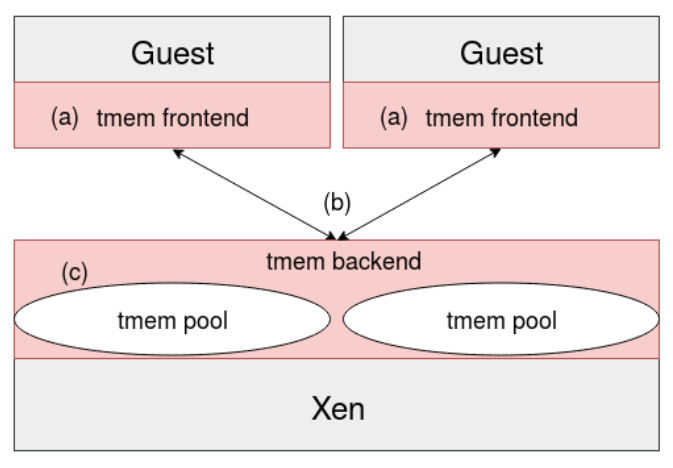
\includegraphics[width=0.5\textwidth]{pictures/tmemXen.PNG}
  \caption{\en{Tmem} επάνω στον \en{Xen hypervisor}}
  \label{fig:tmemXen}
\end{figure}






%UTMEM

\subsection{\en{Userspace transcedent memory - utmem}}

Μέχρι στιγμής ο μηχανισμός \en{tmem}, αφορά περιπτώσεις χρήσης από
υποσυστήματα που τρέχουν «σιωπηλά» εντός του πυρήνα. Ένας
προγραμματιστής, όχι μόνο αγνοεί την ύπαρξη ενός τέτοιου συστήματος,
αλλά ούτε είναι σε θέση να αναπτύξει προγράμματα ικανά να χρησιμοπούν ρητά τον μηχανισμό.
Δημιουργείται, συνεπώς, η
εύλογη απορία αν θα ήταν δυνατόν ένας τέτοιος μηχανισμός να
είναι διαθέσιμος στο \en{user space}.
\newline

Η απάντηση δόθηκε σε μια προηγούμενη διπλωματική εργασία του εργαστηρίου
υπολογιστικών συστημάτων του Εθνικού Μετσοβίου Πολυτεχνείου,
 όπου υλοποιήθηκε ένας τέτοιος μηχανισμός από τον Αιμίλιο Τσαλαπάτη.
Ονομάστηκε \en{utmem} (από το \en{user space tmem}). Αποδείχθηκε,
μάλιστα, πειραματικά πως σε συγκεκριμένες περιπτώσεις πίεσης
μνήμης οι διεργασίες που χρησιμοποιούν αυτόν τον μηχανισμό \en{utmem}
συμπεριφέρονται καλύτερα από διεργασίες που στηρίζονται σε
\en{tmem} μόνο έμμεσα με χρήση του \en{frontswap subsystem}\cite{Aimilios}\cite{paperAimiliou}.
\newline

Η δομή του μηχανισμούς είναι πολύ απλή, και αφορά την επικοινωνία ενός \en{linux guest},
ο οποίος τρέχει επάνω στο \en{KVM}, και ενός \en{linux host}. Αυτή τη
στιγμή, η \en{utmem} συνεργάζεται μόνο με το \en{KVM} ως \en{hypervisor}.
\newline

Αρχικά σχεδιάστηκε μια εικονική συσκευή (\en{virtual device}), που
ονομάστηκε \en{dev/utmem}, η οποία εκθέτει τον μηχανισμό σε διεργασίες
του \en{user space}. Για να τον χρησιμοποιήσει μια διεργασία, πρέπει
αρχικά να ανοίξει την συσκευή (\en{open}), και ύστερα με κλήση
συστήματος \en{ioctl}, να στέλνει αιτήματα στον πυρήνα του λειτουργικού
να αναλάβει να διαχειριστεί κομμάτια από την μνήμη της. Εσωτερικά,
η διεπαφή έρχεται από την αυθεντική \en{tmem} που σχεδίασε η \en{Oracle}. Υπάρχουν ενέργειες
\en{Put} και \en{Get}, για ανταλλαγή δεδομένων, καθώς και \en{Invalidate}
ώστε να ακυρώνονται κλειδιά που αντιστοιχούν σε δεδομένα τα οποία πλέον δεν χρειάζεται
η εφαρμογή.
\newline

Στην συνέχεια, η εσωτερική δομή της συσκευής δέχεται το αίτημα
και τα δεδομένα της διεργασίας και ελέγχει πως όλα είναι σωστά.
Αυτό γίνεται πλέον στον χώρο πυρήνα. Αν ο έλεγχος είναι επιτυχής,
τότε ζητά μέσω κλήση επόπτη (\en{hypercall}), στο \en{backend} να αναλάβει
το αίτημα. Η συσκευή, παρέχει ταυτόχρονα και δευτερεύουσες
λειτουργίες οι οποίες σχετίζονται με την συμπεριφορά της,
με όρια (\en{quota}) που μπορούν να τεθούν στις διεργασίες, και με καταγραφή
στατιστικών για την χρήση του μηχανισμού.
\newline

Τέλος, το \en{backend}, το οποίο έχει ενσωματωθεί στον \en{KVM} επόπτη,
αναλαμβάνει τελικά τα αιτήματα και τοποθετεί δεδομένα σε ένα
\en{pool} στον πυρήνα του \en{host} λειτουργικού.
\newline

Παράλληλα, τροποποιήθηκε το \en{frontswap} υποσύστημα του \en{linux},
ώστε να χρησιμοποιεί τον ίδιο μηχανισμό και \en{backend} με την \en{utmem}
συσκευή, ώστε να είναι εφικτή η αξιοποίηση του νέου \en{backend},
καθώς και η εκτίμηση της αξίας ολόκληρου του μηχανισμού της \en{utmem}.

\begin{figure}[h]
  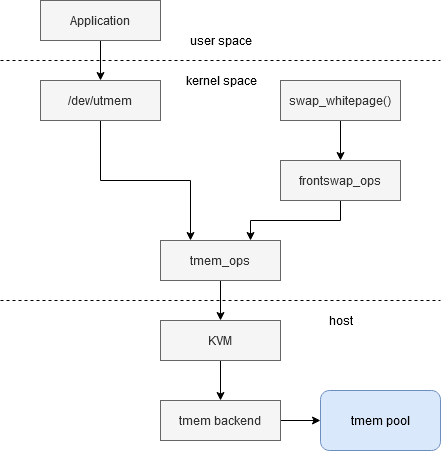
\includegraphics[width=0.7\textwidth]{pictures/utmemFlow.png}
  \caption{Δομή του \en{utmem} μηχανισμού}
  \label{fig:genUtmem}
\end{figure}

\section{Συμπεράσματα - Στόχος της εργασίας}

Πλέον είναι σαφές ότι η \en{utmem} είναι κατάλληλη λύση για περιπτώσεις
\en{virtualization} όπου υπάρχει πίεση μνήμης, ή έχει δοθεί ελάχιστη στο
\en{guest} σύστημα. Η εκτέλεση υπηρεσιών ως \en{unikernels}, είναι ένα συνηθισμένο
παράδειγμα ελάχιστης διαθέσιμης μνήμης, όπου θα ταίριαζε ένας μηχανισμός
ανταλλαγής μνήμης με τον \en{host}, όπως η \en{utmem}. Σκοπός αυτής της εργασίας
είναι να ενσωματώσουμε τον μηχανισμό \en{utmem} στο \en{Rumprun unikernel framework}.
Επίσης, όπως θα φανεί και στην συνέχεια, εκτιμάται η χρηστική αξία και οι επιδόσεις του
συνδυασμού των προαναφερθέντων τεχνολογιών.


\chapter{Σχεδιασμός και υλοποίηση}

Προς αποφυγή παρεξηγήσεων ή παρερμηνειών, εις το εξής θα αναφερόμαστε στον μηχανισμό
\en{utmem} που παρουσιάστηκε στο προηγούμενο κεφάλαιο ως αυθεντικό μηχανισμό
ή αυθεντική \en{utmem}. Στην έκδοση που υλοποιήσαμε και παρουσιάζουμε στην παρούσα
εργασία θα αναφερόμαστε ως \en{unikernel utmem} ή απλά \en{unikernel} έκδοση.

Η αυθεντική υλοποίηση του μηχανισμού \en{utmem} διαχωρίζει τον
μηχανισμό σε τρία αρθρωτά μέρη. Την συσκευή \en{(device) /dev/utmem}, τον χρήστη
\en{utmem} και το πίσω μέρος (\en{backend})\cite{paperAimiliou}. Από αυτά, τα δύο πρώτα
βρίσκονται στο περιβάλλον του \en{guest} και το τρίτο στο περιβάλλον
του \en{host}. Επειδή τα μέρη αυτά είναι εκ κατασκευής σε αρκετά
υψηλό βαθμό ανεξάρτητα μεταξύ τους, και επειδή ο \en{host} θα
παραμένει ένα παραδοσιακό \en{POSIX} λειτουργικό σύστημα (\en{linux})
διατηρούμε αυτούσιο το πίσω μέρος ως έχει, ενώ προσαρμόζουμε
τα άλλα δύο μέρη στο \en{unikernel} περιβάλλον. Επίσης, αγνοούμε
μερικά άλλα τοπικά \en{backend}, που προσφέρονται στο \en{repository}
της αυθεντικής \en{utmem} καθώς χρησιμεύουν μόνο ως δοκιμές και δεν
συνεργάζονται με τον \en{host}. Ο επόπτης (\en{hypervisor})
παραμένει το \en{KVM} όπως και στην αυθεντική υλοποίηση.
\newline

Θυμίζουμε πως η συσκευή \en{utmem} εκτός των βασικών λειτουργιών,
προσφέρει μέσω την \en{ioctl} κλήσης μια πληθώρα βοηθητικών
λειτουργιών οι οποίες έχουν να κάνουν με δευτερεύουσες
επιλογές και αξιοποίηση μετρητικών ενδείξεων. Επειδή μας
ενδιαφέρει η περίπτωση της επικοινωνίας \en{host} και \en{guest}, η
υλοποίηση για \en{unikernel} περιβάλλον υποστηρίζει μόνο τις
βασικές, αλλά συνάμα απαραίτητες, λειτουργίες επάνω στην πτητική
μνήμη (\en{Get}, \en{Put}, \en{Invalidate})
και συνεπώς επιλέγουμε να απουσιάζουν οι προαναφερθείσες δευτερεύουσες λειτουργίες.
\newline

Η ενσωμάτωση του μηχανισμού \en{utmem} στο \en{Rumprun} έγινε σε δύο φάσεις,
με δυο διαφορετικές μορφές.
Αμφότερες αναλύονται στην συνέχεια, ενώ και οι δύο μπορούν
αξιόπιστα να επιτελέσουν τις τρεις βασικές λειτουργίες \en{utmem}
που μας ενδιαφέρουν.
\newline

Επίσης, εις το εξής θα αναφερόμαστε στα \en{user space} και \en{kernel space}
με εισαγωγικά («\en{user space}» - «\en{kernel space}»), θέλοντας να
δείξουμε την αντιστοιχία, ως προς το επίπεδο της στοίβας
λογισμικού του \en{Rumprun}, με τους αντίστοιχους χώρους που υπάρχουν στα
συμβατικά λειτουργικά.
\newline

Τέλος, αναφέρουμε η πως μεταφορά δεδομένων στην \en{utmem} γίνεται
χρησιμοποιώντας το \en{struct tmem\_request }. Αυτό πρόκειται για
ένα \en{datatype}, με το οποίο μπορούμε να αντιγράψουμε μεταξύ
\en{host} και \en{guest} μνήμη (\en{value}) αυθαίρετου μεγέθους, η οποία
αναφέρεται με κλειδί (\en{key}) επίσης αυθαίρετου μεγέθους. Για να
έχουμε συμβατότητα με τον αυθεντικό μηχανισμό διατηρούμε και
εμείς τα ίδια \en{semantics} και \en{data types}.
\newline

\begin{figure}[h]
  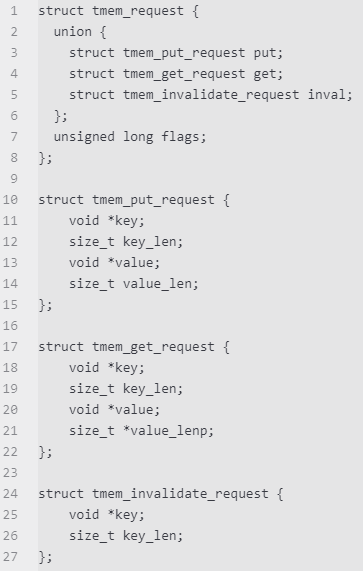
\includegraphics[height=0.4\paperheight]{pictures/struct2.PNG}
  \caption{Το \en{struct tmem\_request } καθώς και δευτερεύοντα
  \en{datatypes} που χρησιμοποιούνται για την μεταφορά δεδομένων}
  \label{fig:structure}
\end{figure}


%syscall
\section{Πρώτη φάση - \en{system call}}

Στο \en{Rumprun} απουσιάζει ο διαχωρισμός των
χώρων χρήστη και χώρο πυρήνα ,
ωστόσο κατά την αρχική υλοποίηση διατηρούμε αυτόν τον , τουλάχιστον
δομικό, διαχωρισμό ώστε η υλοποίηση να μοιάζει περισσότερο με την
αυθεντική υλοποίηση της \en{utmem} σε \en{linux}. Προς αποφυγή
οποιασδήποτε παρεξήγησης,
δεν εννοούμε πως
δημιουργούμε ξεχωριστό χώρο διευθύνσεων, αλλά πως εισάγουμε την
\en{utmem} χαμηλά στην στοίβα λογισμικού, εκεί που παραδοσιακά βρίσκεται
ο χώρο του πυρήνα. Συνεπώς, με βάση αυτήν μας την επιλογή μια «\en{user space}»
εφαρμογή στο \en{Rumprun}, εφόσον
επιθυμεί να χρησιμοποιήσει τις \en{utmem} λειτουργίες, οφείλει να ζητήσει
από τον πυρήνα να εκτελέσει τις λειτουργίες αυτές εκ μέρους της,
θεωρώντας πως δεν έχει την ικανότητα να την επιτελέσει η ίδια στο «\en{user space}».
\newline

Στην αυθεντική υλοποίηση του \en{utmem} μηχανισμού προστέθηκε μια \en{virtual device}
στο λειτουργικό, την οποία οι εφαρμογές χρησιμοποιούσαν μέσω \en{ioctl}
κλήσεις συστήματος. Στην \en{Rumprun} υλοποίηση προσθέσαμε απλά μια
νέα κλήση συστήματος \en{(system call)} του \en{NetBSD} , την οποία ονομάσαμε
\en{tmem} με αριθμό 483, η οποία υποστηρίζει τις τρεις βασικές λειτουργίες
(\en{operations}) της \en{utmem} με βάση το \en{KVM}, δηλαδή \en{Put, Get, Invalidate}.
Αυτή η κλήση συστήματος αντικαθιστά την χρήση της \en{ioctl} από
την εφαρμογή. Εν τέλει, η κλήση συστήματος θα μεταφραστεί
σε κλήση συνάρτησης από τα \en{rump kernels}, όταν δημιουργηθεί το
τελικό \en{unikernel}. Για να γίνει αυτό, φροντίσαμε να ενημερώσουμε
τα \en{rump kernels} για την ύπαρξη αυτής της νέας κλήσης συστήματος, έτσι
ώστε κατά το \en{build} του \en{toolchain} να συμπεριληφθεί , ώστε στην
συνέχεια να είναι διαθέσιμη κατά το \en{bake} των \en{unikernel}.
\newline

Επιλέξαμε την εισαγωγή της νέας κλήσης συστήματος καθώς από πλευράς έκτασης
κώδικα και χρήσης από
μια «\en{user space}» εφαρμογή είναι απλούστερο από το να εισάγουμε
μια εικονική συσκευή όπως στην αυθεντική \en{utmem}. Μην ξεχνάμε
πως βασική φιλοσοφία των \en{unikernels} είναι η ελαχιστοποίηση
του αποτυπώματος των εφαρμογών που εκτελούνται. Άλλωστε, δεν αποτελεί
την τελική μορφή όπως θα φανεί και στην συνέχεια.
\newline

Η ροή των ενεργειών που θα ακολουθηθεί όταν μια
εφαρμογή-\en{unikernel} επιθυμεί να αποθηκεύσει στον \en{host}
ένα κομμάτι της μνήμης του στον \en{guest}, μέσω του \en{operation} \en{Put}, είναι η εξής:
\begin{enumerate}
  \item Η εφαρμογή γεμίζει μια περιοχή μνήμης της με δεδομένα.
  Αυτά τα δεδομένα σκοπεύει να τα δώσει στον \en{host}, ώστε να μπορεί να στη συνέχεια
  να αποδεσμεύσει αυτήν την περιοχή μνήμης.

  \item Εκτελεί την κλήση συστήματος \en{tmem}, όπου δηλώνει
  την διεύθυνση μνήμης της περιοχής, το όνομα του κλειδιου
  με το οποίο θα αναφερόμαστε σε αυτή, και το μέγεθος της. Η
  ροή περνά στο «\en{kernel space}».

  \item O πυρήνας αντιγράφει τα δεδομένα σε δικό του χώρο,
  ελέγχει πως όλα είναι σωστά, και εκτελεί το \en{KVM hypercall}
  που αφορά την \en{tmem} και συγκεκριμένα το \en{Put operation}.

  \item Το \en{backend} λαμβάνει το \en{hypercall request} και
  αναλαμβάνει να αποθηκεύσει την μνήμη που ζητήθηκε. Η
  συμπεριφορά του είναι ίδια με την περίπτωση που
  είχαμε \en{virtualized guest} ως κανονικό λειτουργικό. Το \en{backend}
  δεν είναι σε θέση να γνωρίζει το είδος της εικονικής μηχανής που έστειλε το
  αίτημα.

  \item Εφόσον όλα πήγαν καλά, επιστρέφεται μήνυμα επιτυχίας
  στον \en{guest} μέχρι και το «\en{user space}» επίπεδο. Πλέον η
  εφαρμογή μπορεί να αποδεσμεύσει την μνήμη.

\end{enumerate}

Η ροή για τα \en{Put} και \en{Invalidate operation} είναι αντίστοιχη με τα παραπάνω.
\newline






\subsection{Τεχνικές δυσκολίες}
Όπως ήταν αναμενόμενο, για να υλοποιηθεί το παραπάνω εμφανίστηκαν
μερικές τεχνικές δυσκολίες.
\newline

Η πρώτη τεχνική δυσκολία στην υλοποίηση του μηχανισμού επικοινωνίας με
τον \en{KVM hypervisor}, και άρα και με τις \en{paravirtualization} ευκολίες
που προσφέρει, είναι πως στο \en{NetBSD} δεν υπάρχει έτοιμος μηχανισμός
(\en{API}) ώστε να εκτελούνται \en{hypercalls} με βάση το \en{KVM} ως \en{hypervisor}.
Αντίθετα στο \en{linux} αυτό το \en{task} είναι πιο απλό. Εκεί υπάρχουν έτοιμες
συναρτήσεις του χώρου πυρήνα\cite{KVMhyper},
ονόματι \en{kvm\_hypercall}Χ,  όπου Χ+1 ο αριθμός των \en{argument} που πρέπει να
γνωρίζει ο \en{host} για την εξυπηρέτηση της \en{hypercall}. Ο \en{tmem} μηχανισμός
για \en{hypercall}  χρειάζεται τρια \en{arguments}, τον κωδικό της \en{tmem}, τον
κωδικό του \en{tmem operation}, και το \en{tmem request structure} το οποίο
εκθέτουμε στον \en{host} ως ανταλλακτήριο πληροφοριών.
\newline

Η λύση στο πρόβλημα αυτό είναι να εξάγουμε από το \en{source tree} του \en{linux} τις
απαραίτητες γραμμές και να τις προσθέσουμε στην κλήση συστήματός μας.
Αυτό αυτομάτως περιορίζει την υλοποίησή μας σε αρχιτεκτονική \en{x}86,
η οποία, όμως, είναι η πλέον δημοφιλής και άρα δεν αποτελεί
μεγάλο μειονέκτημα. Ακολουθήσαμε λοιπόν την ροή της \en{kvm\_hypercall2}
στο \en{linux}, και καταλήγουμε σε περίπου 60 γραμμές \en{x}86 \en{assembly}. Το
πιο σημαντικό εντός αυτών είναι πως εκτελείται ένα \en{X86\_FEATURE\_VMMCALL} με
νούμερο (8*32+15) το οποίο όπως αναμενόταν αφορά το \en{KVM hypervisor}
στην \en{x}86 αρχιτεκτονική. Παίρνοντας αυτές τις γραμμές από τον
πηγαίο κώδικα του \en{linux} και τοποθετώντας τες σε ένα \en{header file},
η \en{system call} που υλοποιούμε είναι σε θέση να καλεί \en{KVM hypercalls}
ακόμα και ως \en{Rumprun unikernel}.
\newline

Το επόμενο βήμα είναι να καλέσουμε \en{KVM hypercall} για
χρήση της \en{utmem} συγκεκριμενα. Τα \en{operation codes} και \en{type code} της \en{utmem}
είναι γνωστά από την αυθεντική υλοποίηση και μπορούν να μεταφερθούν αυτούσια.
\newline

Εδώ εμφανίζεται και η δεύτερη τεχνική δυσκολία, η οποία
είναι η έκθεση (\en{expose}) των πληροφοριών μας στον \en{host} που
αναλαμβάνει την εξυπηρέτηση των \en{hypercall} μας. O μηχανισμός
\en{utmem} χρησιμοποιεί \en{instances} του \en{tmem\_request struct} ώστε να
μεταφέρεται η πληροφορία από τον \en{host} στον \en{guest} ή ανάποδα.
Το συγκεκριμένο \en{struct} φέρει την τιμή του ζευγαριού \en{key-value}
καθώς και βοηθητικές πληροφορίες που έχουν να κάνουν με το μέγεθος
της εκάστοτε τιμής. Δυστυχώς ο \en{host} και ο \en{guest} «ζουν» σε
διαφορετικούς χώρους μνήμης (\en{memory space}) και χρειάζεται μετάφραση
σε φυσικό χώρο διευθύνσεων (\en{physical address space}), τον οποίο
ο \en{host} είναι σε θέση να προσπελάσει. Η αυθεντική υλοποίηση της \en{utmem}
μεταφράζει \en{page-aligned virtual addresses} σε \en{physical address}. Η
ευθυγράμμιση σε επίπεδο σελίδας (\en{page alignment}) δεν είναι
απαραίτητη και φαίνεται πως είναι κατάλοιπο από τα αρχικά στάδια
της υλοποίησης του μηχανισμού της \en{utmem}, οπότε επιλέξαμε να την
αγνοήσουμε στην δική μας υλοποίηση. Τονίζουμε πως αυτό δεν επηρεάζει την ορθή
επικοινωνία μεταξύ των δύο πλευρών. Για να επιτύχουμε την μετάφραση από
\en{virtual address} σε \en{physical address} χρησιμοποιούμε την
συνάρτηση \en{vtophys}() που προσφέρει το \en{NetBSD} σε χώρο πυρήνα,
ενώ παράλληλα την υποστηρίζουν και τα \en{rump kernels}.
\newline

Υλοποιήσαμε συνεπώς ό,τι χρειάζεται η \en{system call} μας και
πλέον έχουμε ένα μηχανισμό αντίστοιχο με της αυθεντικής υλοποίησης
της \en{utmem}, ο οποίος μπορεί να χρησιμοποιηθεί σε \en{unikernel}
περιβάλλον. Όλος ο κώδικας δεν ξεπερνά τις 450 γραμμές,
αρκετές από τις οποίες είναι αντίγραφα κώδικα του πυρήνα
του \en{Linux} και δεν έχουν γραφτεί από εμάς.

\begin{figure}[h]
  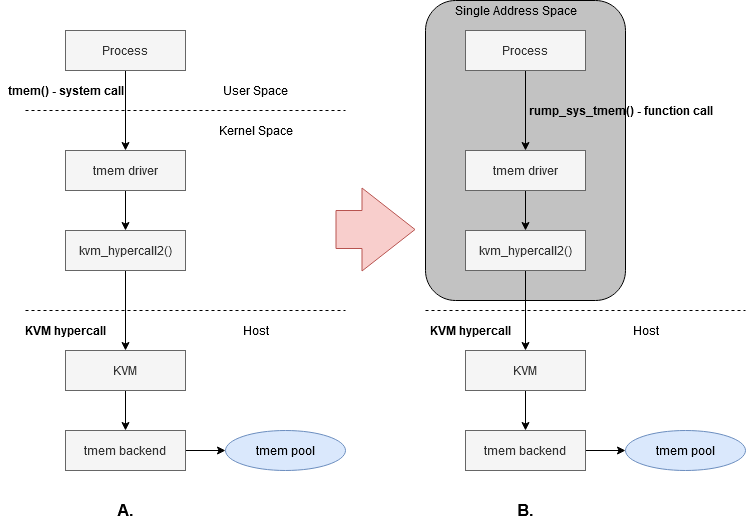
\includegraphics[width=\textwidth]{pictures/syscallFlow.png}
  \caption{Α.Ροή εκτέλεσης της \en{system call tmem()} στο \en{NetBSD}
   Β. H μετατροπή της σε \en{function call} από τα \en{rump kernels}}
  \label{fig:syscallFlow}
\end{figure}




\section{Δεύτερη φάση - \en{function call}}

Όπως αναφέραμε, στο \en{Rumprun} υπάρχει μόνο ένας χώρος διευθύνσεων
καθώς εφαρμογή και πυρήνας γίνονται \en{bake} σε ένα σώμα, το
\en{unikernel}. Ως εκ τούτου, η αρχική μας προσέγγιση διαχωρισμού είναι κενή σημασίας,
απλά βοηθά στην καλύτερη κατανόηση της ροής αφού θυμίζει
περισσότερο παραδοσιακό περιβάλλον. Θα ήταν σαφώς καλύτερο να
εκμεταλλευτούμε την χαρακτηριστική αυτή ιδιότητα ώστε η υλοποίησή μας να
έχει ελάχιστο αποτύπωμα στο περιβάλλον ανάπτυξης.
\newline

Με μια προσεχτική ματία στον κώδικα, η μόνη εξάρτηση από συνάρτηση του πυρήνα,
αντίστοιχη της οποίας δεν υπάρχει σε χώρο χρήστη, είναι για
την μετάφραση από \en{virtual} σε \en{physical addresses} μέσω της
\en{vtophys}(). Η υλοποίηση αυτής στα \en{rump kernels} είναι εξαιρετικά
απλή, το οποίο μας επιτρέπει την αντιγράψουμε
σε «\en{user space}» επίπεδο, δηλαδή στα ανώτερα στρώματα της στοίβας του λογισμικού.
Παίρνουμε λοιπόν ό,τι χρειάζεται και για την εκτέλεση του
\en{hypercall} και πλέον μπορούμε να έχουμε όλη τη λειτουργικότητα
της \en{utmem} δίχως την ανάγκη μιας \en{system call}. Δημιουργήσαμε μια
βιβλιοθήκη, έτοιμη να συμπεριληφθεί στον κώδικα από οποιοδήποτε πρόγραμμα το
επιθυμεί. Ό,τι κάναμε πριν εντός της \en{system call} το κάνουμε τώρα
σε ένα «\en{user space}» \en{.c file}, το οποίο ως σχεδίαση είναι σαφώς
απλούστερο από πριν.
\newline

Από την μια, η ανάπτυξη εφαρμογών γίνεται ελαφρώς πιο σύνθετη, καθώς
πρέπει να προστεθεί κατά το \en{linking} αυτών και ο κώδικας
που εκτελεί τα \en{hypercall} και προσφέρει τα \en{utmem operations},
σε αντίθεση με την \en{system call} όπου η \en{libc} αναλαμβάνει την
αντιστοιχία. Από την άλλη, όμως, το κέρδος είναι πως πλέον δεν απαιτούνται
αλλαγές στο \en{Rumprun-rump kernels}. Η τελική μορφή των δύο εκδώσεων διαφέρει ελάχιστα,
καθώς η \en{system call tmem} της πρώτης φάσης
εν τέλει μεταφράζεται σε ένα απλό \en{function call} από το \en{Rumprun},
με αποτέλεσμα το \en{overhead} να είναι ίδιο στις δύο περιπτώσεις. Μια μικρή διαφορά
είναι πως η function call απαιτεί μια αντιγραφή λιγότερη των δεδομένων.
\newline

Συντονιζόμαστε, συνεπώς, με την φιλοσοφία πίσω από τα \en{rump kernels},
δηλαδή την ανάπτυξη και εκτέλεση \en{drivers} από τον χώρο χρήστη,
δίχως να απαιτείται η προσαρμογή του υφιστάμενου πυρήνα. Ο \en{driver}
μας είναι όλος ο κώδικας που αναλαμβάνει να εκτελέσει την κλήση
επόπτη, και να ανταλλάξει με ασφάλεια τα κομμάτια μνήμη μεταξύ
του \en{guest} και του \en{host}.

\begin{figure}[h]
  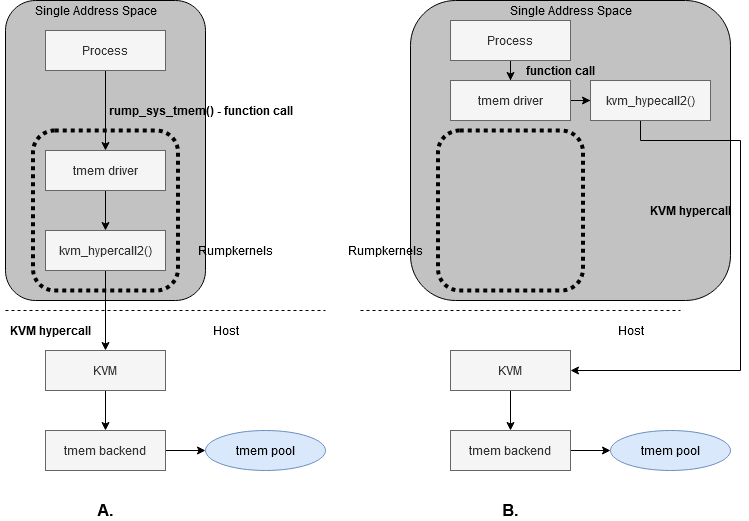
\includegraphics[width=\textwidth]{pictures/sys-func_diff.png}
  \caption{A.\en{Utmem} στο \en{Rumprun} ως \en{system call}
   Β. \en{Utmem} στο \en{Rumprun} ως \en{function call}}
  \label{fig:syscall_funcall}
\end{figure}


\chapter{Αξιολόγηση επιδόσεων}

\section{Σύγκριση με υπάρχουσες \en{unikernel} λύσεις}

Για την αξιολόγηση του μηχανισμού \en{utmem} ως \en{unikernel}
χρησιμοποιούμε ως καταλληλότερο το μετροπρόγραμμα (\en{benchmark)}
\en{Redis (Remote Dictionary Server)}.
Το \en{Redis} είναι ιδανικό για αυτόν το σκοπο για δύο
λόγους. Πρώτον πρόκειται, όπως λέει και ίδιο \cite{redis}, για ένα
\en{data structure store}, δηλαδή ένα εξυπηρετητή αποθήκευσης αφηρημένων
δεδομένων, όπου οι βασικές λειτουργίες είναι \en{get} και \en{set}
με αναφορά σε κλειδιά, και άρα υπάρχει προφανής ομοιότητα
με τα \en{utmem operations}. Δεύτερον, υπάρχει ήδη έκδοση \en{unikernel}
του \en{Redis} από τα προσφερόμενα \en{Rumprun-packages} στο επίσημο \en{repository},
οπότε δεν χρειάζεται να το μετατρέψουμε εμείς σε \en{unikernel}\cite{redisUni}.
\newline

Η γενική δομή του \en{Redis} μοντέλου, είναι η ύπαρξη ενός \en{back-end server},
ο οποίος είναι υπεύθυνος για την αποθήκευση αφηρημένης
μορφής δεδομένων, και την εξυπηρέτηση αιτημάτων από τρίτες
εφαρμογές επάνω σε αυτά τα δεδομένα. Ταυτόχρονα, υπάρχουν
διάφοροι \en{front-end clients}, οι οποίοι αποστέλνουν αιτήματα
στον server με το \en{TCP/IP} πρωτόκολλο. Ως \en{unikernel}
προσφέρεται μόνο ο \en{Redis server}, και ο \en{client} μπορεί να
είναι οποιαδήποτε εφαρμογή ικανή να διαχειρίζεται \en{TCP} αιτήματα, π.χ. \en{nc}.
\newline

Αποφασίζουμε να προσθέσουμε τρεις νέες εντολές στο\en{ Redis},
τις \en{tmemPut, tmemGet, tmemInval},
οι οποίες όπως δείχνει το ονομά τους αντιστοιχούν
στα τρια \en{utmem operation} που υλοποιήσαμε. Στα εξής θα
αναφερόμαστε σε αυτές τις εντολές ως \en{tmem commands},
για να τις ξεχωρίζουμε από τα \en{tmem operations}. Ο προτεινόμενος
τρόπος εισαγωγής εντολών στο \en{Redis} είναι η δημιουργία
ενός \en{Redis module} το οποίο προσθέτει τις εντολές κατά
το \en{runtime} του \en{Redis server}. Όμως η έκδοση του \en{Redis},
που υπάρχει ως \en{unikernel}, είναι αρκετά παλιά και δεν
υποστηρίζει τα \en{modules}, οπότε προσθέσαμε τις εντολές απευθείας
στον πηγαίο κώδικα του \en{Redis server}.
\newline

Επίσης επιλέγουμε να χρησιμοποιηθεί η έκδοση \en{utmem} μέσω
\en{function call}, και όχι \en{system call}. Αυτό εξαλείφει
την πιθανότητα τα αποτελέσματά μας να επηρεάζονται από
τις αλλαγές στα \en{rump kernels}, μιας και τα χρησιμοποιούμε
χωρίς αλλαγή. Πρέπει μόνο να ενσωματώσουμε την
μεταγλώττιση του\en{ driver} της \en{utmem} στο \en{Redis}, το οποίο
σημαίνει να προστεθούν \en{flags} για \en{assembly compilation}.
\newline

Οι μετρήσεις έγιναν μέσα σε εικονική μηχανή \en{QEMU/KVM}
με \en{Ubuntu Linux 4.9.39}, στον πυρήνα του οποίου
έχουν προστεθεί τα \en{patch} της αυθεντικής \en{utmem} για το
\en{back-end}. Ο επεξεργαστής είναι \en{intel core i5-8250u} από τον οποίο
αναθέτουμε 2 φυσικούς πυρήνες (4 λογικούς), ενώ η
διαθέσιμη μνήμη \en{RAM} του \en{VM} είναι \en{4GB}.
\newline

Τέλος, οφείλουμε να διευκρινίσουμε πως εκτελουμε το
\en{Redis} χωρίς \en{AOF persistence}. Το \en{Redis} προσφέρει
δυνατότητα διατήρησης των δεδομένων της μνήμης τους
στο δίσκο ώστε αυτά να μπορούν να ανακτηθούν σε περίπτωση
μη προβλεπόμενου τερματισμού του \en{Redis}. Διατηρεί,
συνεπώς ένα αρχείο με αυτές τις εγγραφές στον δίσκο.
Το μειονέκτημα, όπως είναι πως κάθε προσθετοαφαίρεση
δεδομένου, π.χ. μια \en{set}, μπλοκάρει μέχρι να γραφούν τα
δεδομένα στο δίσκο\cite{redisAOF}. Ως γνωστόν, οι δίσκοι είναι τάξης
μεγέθους πιο αργοί από την κύρια μνήμη, συνεπώς το να
διατηρούσαμε το \en{AOF persistance} του \en{Redis} θα έδινε ένα
άδικο πλεονέκτημα στα \en{tmem commands} μας, τα οποία δεν
διατηρούν τέτοια αντίγραφα. Συγκρίνουμε, λοιπόν μόνο
\en{in-memory} ενέργειες του \en{Redis}.



\subsection{Σενάριο 1: με άφθονη μνήμη}

Για μετρήσουμε την συμπεριφορά του \en{Redis} με τα νέα \en{commands},
δημιουργήσαμε ένα \en{custom} μετροπρόγραμμα, το οποίο ονομάζουμε
\en{client}. Το πρόγραμμα αποστέλνει μέσω \en{TCP/IP network requests},
προς το \en{Redis}. Ταυτόχρονα, ο client καταγράφει δεδομένα για την επίδοση
της επικοινωνίας με τον \en{server}. O \en{client} τρέχει στον \en{host} ως απλή διεργασία
ώστε να μην επηρεάζεται η εκτέλεση του \en{Redis}, το οποίο
με την σειρά του τρέχει ως \en{unikernel}. Θέλουμε να συγκρίνουμε
δύο \en{commands}, το απλό \en{set} και το \en{tmemPut}, οπότε για δίαφορους
συνδυασμούς μεγέθους \en{value} και αριθμό \en{requests} λαμβάνουμε
μετρήσεις για το πόσο χρόνο χρειάστηκε να ικανοποιηθούν όλα
τα \en{requests}, και στην συνέχεια παίρνουμε ένα μέσο όρο.
Συνεπώς, η μετρική που μας ενδιαφέρει είναι τα \en{commands}/δευτερόλεπτο.
\newline

Αναλυτικότερα, επιλέγουμε ένα μέγεθος τιμής (\en{value size}) και ένα αριθμό από
τιμές (\en{number of values}) που θα καταχωρήσουμε στο \en{Redis}.
Για παράδειγμα ο συνδυασμός 512-1024 σημαίνει πως θα
καταχωρηθούν 1024 τιμές, η κάθε μια από τις οποίες αντιστοιχεί σε ένα ξεχωριστό command,
όπου κάθε τιμή θα έχει μέγεθος 512 bytes. Αυτή η διαδικασία γίνεται για πολλούς συνδυασμούς
\en{value size} και \en{number of values}. Προφανώς, ανάμεσα σε κάθε επανάληψη του πειράματος φροντίζουμε
να αδειάζει η μνήμη του \en{Redis} ή το \en{tmem pool}, για
το \en{set} ή το \en{tmemPut} αντίστοιχα.
\newline

Η δομή του συστήματος \en{client} και \en{Redis unikernel} φαίνεται στην εικόνα
\ref{fig:benchSetup}.
\newline

\begin{figure}[h]
  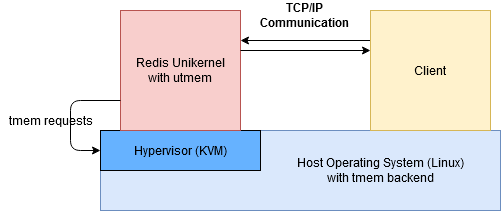
\includegraphics[width=\textwidth]{pictures/benchmarkSetup.png}
  \caption{Επικοινωνία και δομή \en{client - Redis unikernel}}
  \label{fig:benchSetup}
\end{figure}

Εν τέλει παρατηρείται πως, όταν υπάρχει αρκετή μνήμη τα \en{tmem commands} είναι σχετικά
πιο αργά από τις \en{set} εντολές του \en{Redis}. Αυτό είναι λογικό,
καθώς πρώτον πρέπει για κάθε \en{tmem command} να
εκτελείται ένα \en{hypercall}, το οποίο είναι σύγχρονος μηχανισμός
και άρα οδηγεί σε μπλοκάρισμα του \en{unikernel}. Δεύτερον, πρέπει
να αντιγράφεται το σύνολο των δεδομένων από τον χώρο του
\en{unikernel} στον χώρο πυρήνα του \en{host}, αυξάνοντας τις αντιγραφές που
εκτελούνται ανά \en{command}. Στην εικόνα \ref{fig:tmemPut-Set} φαίνεται
η σχετική συμπεριφορά των δύο ειδών \en{commands} για διάφορους συνδυασμούς μεγέθους \en{value}
και αριθμού \en{requests}, ενώ στην εικόνα \ref{fig:tmemPut-SetPercentage} παρουσιάζεται η ποσοστιαία
διαφορά ταχύτητας των δύο εντολών παίρνοντας μέσο όρο ανά \en{value size}.
\newline

\begin{figure}[h]
  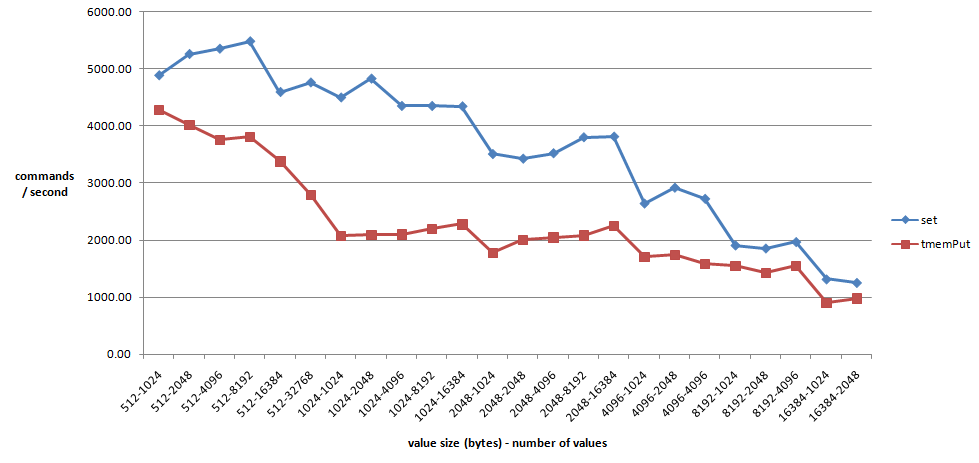
\includegraphics[width=\textwidth]{pictures/firstBenchmarkResults.PNG}
  \caption{Σύγκριση \en{tmemPut} και \en{set commands}. Φαίνεται πως
  η \en{tmemPut} σχετικά πιο αργή από την \en{set} μετρώντας
  \en{commands/second}}
  \label{fig:tmemPut-Set}
\end{figure}

\begin{figure}[h]
  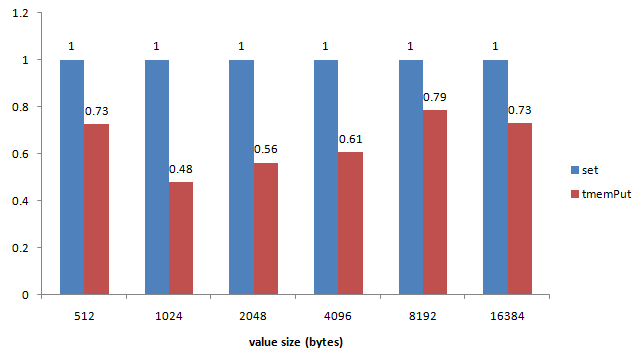
\includegraphics[width=\textwidth]{pictures/firstBenchmarkResults2.PNG}
  \caption{Ποσοστιαία σχέση \en{tmemPut} και \en{set} κανονικοποιημένη ως προς \en{set}}
  \label{fig:tmemPut-SetPercentage}
\end{figure}


\subsection{Σενάριο 2: με έλλειψη μνήμης}

Επιθυμούμε να μελετήσουμε την συμπεριφορά του \en{Redis} και σε περιπτώσεις
όπου ο πόρος της μνήμης είναι σημαντικά περιορισμένος. Τρέχουμε πάλι τον ίδιο
\en{Unikerel server}, αλλά τώρα περιορίζουμε την διαθέσιμη μνήμη όλης της εικονικής
μηχανής σε μερικές δεκάδες \en{mega bytes}.
\newline

Όταν η μνήμη είναι περιορισμένη, τα \en{tmem commands} γίνονται η
μόνη λειτουργική λύση για αποθήκευση δεδομένων. Θυμίζουμε
πως στο \en{Rumprun} απουσιάζει η εικονική μνήμη, συνεπώς όταν
γεμίσει η διαθέσιμη δεν υπάρχει κάποιος μηχανισμός να απελευθερώσει
αυτήν την πίεση μνήμης. Στην περίπτωση του \en{set}, μετά από ένα
αριθμό από \en{requests}, είναι αδύνατον να κατανεμηθεί νέα μνήμη, έστω
εικονική, στο \en{Redis}, το οποίο πλέον αδυνατεί να ικανοποιήσει
τα \en{requests} που του έρχονται από τον \en{client}. Σε αυτό το σενάριο, εμφανίζει
μήνυμα σφάλματος και τερματίζει την λειτουργία του. Καταστροφική
συμπεριφορά για ένα εξωτερικό χρήστη που επικοινωνεί με το
\en{unikernel}. Αντίθετα, το \en{tmemPut} ικανοποιείται κανονικά, καθώς η
απαίητηση σε χώρο είναι ελάχιστη, αρκεί δηλαδή να ικανοποιείται
ένα \en{request}, για να ικανοποιηθούν όλα, μιας και τα δεδομένα
αποθηκεύονται στην μνήμη του \en{host}. Μάλιστα η συμπεριφορά είναι
ταυτόσημη με την περίπτωση αφθονίας μνήμης, δεν παρατηρείται κάμια επιπλέον
καθυστέρηση λόγω της περιορισμένης μνήμης.







\section{Σύγκριση με την αυθεντική \en{utmem}}

Για να εξαχθεί μια πλήρης εικόνα των επιδόσεων του μηχανισμού, θεωρούμε σκόπιμο,
να συγκρίνουμε την \en{utmem} υλοποίηση σε \en{unikernel}, σε σχέση με τον
αυθεντικό (\en{original}) μηχανισμό της \en{utmem}.
\newline

Χρησιμοποιούμε πάλι το μετροπρόγραμμα \en{Redis}, για το οποίο υπάρχει
\en{Redis-module} με το οποίο το \en{Redis} τίθεται ικανό να ικανοποιήσει \en{utmem}
αιτήματα χρησιμοποιώντας τον αυθεντικό μηχανισμό. Αναφερόμαστε πλέον στο
\en{Redis} ως κανονική διεργασία ενός \en{linux} συστήματος. Θυμίζουμε, πως ο
αυθεντικός μηχανισμός χρησιμοποιεί μια εικονική συσκευή (\en{/dev/utmem}) του \en{linux},
ούτως ώστε οι διεργασίες να μπορούν να ζητάν από τον πυρήνα να
εκτελέσει \en{tmem} αιτήματα προς το \en{backend} εκ μέρους αυτών. Επιπροσθέτως,
επιθυμούμε ο τρόπος μέτρησεις να είναι όσο το δυνατόν όμοιως με τον τρόπο
μέτρησης που περιγράφεται στην εργασία της αυθεντικής \en{utmem} \cite{Aimilios}, συνεπώς
δημιουργήσαμε ένα διαφορετίκό πρόγραμμα \en{client} που αποστέλει αιτήματα. Αυτή τη φορά,
δεν γεμίζουμε την \en{tmem pool} με δεδομένα, αλλά αποστέλλουμε συνεχώς το ίδιο αίτημα,
δηλαδή το ίδιο \en{key}, για προκαθορισμένο χρονικό διάστημα και εν τέλει υπολογίζουμε ένα
μέσο όρο αιτημάτων. Αποστέλουμε ακριβώς τα ίδια αιτήματα και στο \en{unikernel Redis}, ωστέ
να μπορούμε να έχουμε μια όμοια σύγκριση μεταξύ των δύο εκδόσεων. Ελέγχουμε διάφορες τιμές του μεγέθους της τιμής (\en{value size}),
ενώ το \en{utmem command} είναι τύπου \en{Put}. Όπως και προηγουμένως, η μετρική που
μας ενδιαφέρει είναι τα \en{commands / second} που εξυπηρετούνται.
\newline

Η τοπολογία του συστήματος μετρήσεων είναι η εξής:
όταν μετράμε την αυθεντική \en{utmem}, το \en{Redis} εκτελείται ως μια
κανονική διεργασία εντός εικονικής μηχανής (\en{guest}) με 2 \en{GB RAM} και ίδιου
πυρήνα με τον \en{host}, δηλαδή τον πυρήνα με τα \en{utmem patches}. Για την \en{utmem}
ως \en{unikernel}, εκτελούμε ένα \en{unikernel} επάνω στον ίδιο \en{host}.
Τέλος, ο \en{client} εκτελείται επίσης ως απλή διεργασία
επάνω στον \en{Ηost}. Η διάταξη φαίνεται καλύτερα στο σχήμα \ref{fig:original-unikernelTopo}.
\newline

\begin{figure}[h]
  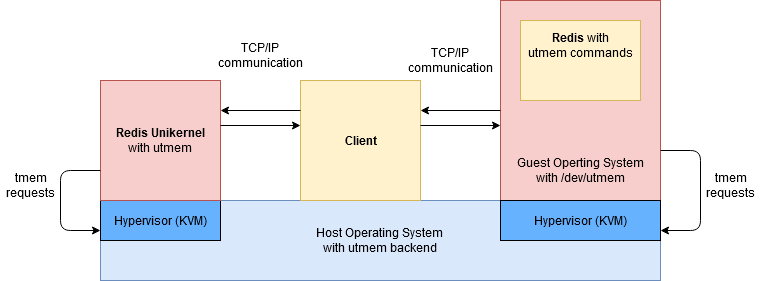
\includegraphics[width=\textwidth]{pictures/bench2Setup.PNG}
  \caption{Τοπολογία σύγκρισης αυθεντικής \en{utmem} και \en{Unikernel utmem}}
  \label{fig:original-unikernelTopo}
\end{figure}

Στο σχήμα \ref{fig:original-unikernel} φαίνονται τα αποτελέσματα των μετρήσεων. Παρατηρούμε
πως η έκδοση \en{utmem} για \en{unikernel} είναι σταθερά ταχύτερη από τον αυθεντικό
μηχανισμό. Μάλιστα, όσο το
μέγεθος του \en{value} μεγαλώνει τόσο η μεγαλώνει και η διαφορά στην επίδοση
ανάμεσα στους δύο μηχανισμούς.
Στο σχήμα \ref{fig:original-unikernelPercentage}
φαίνεται και η ποσοστιαία διαφορά των δύο εκδόσεων ανά \en{value size}.
\newline

\begin{figure}[h]
  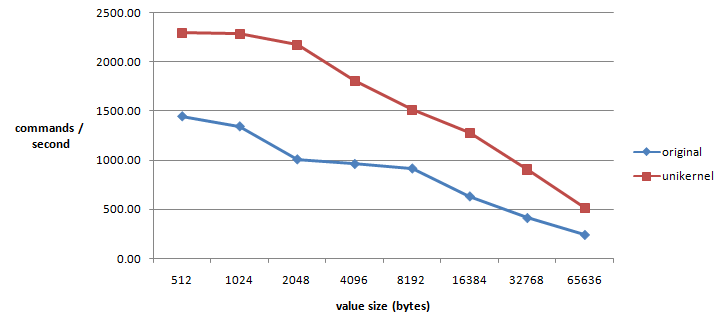
\includegraphics[width=\textwidth]{pictures/secondBenchmarkResults.PNG}
  \caption{Επίδοση αυθεντικής \en{utmem} και \en{Unikernel utmem}}
  \label{fig:original-unikernel}
\end{figure}

\begin{figure}[h]
  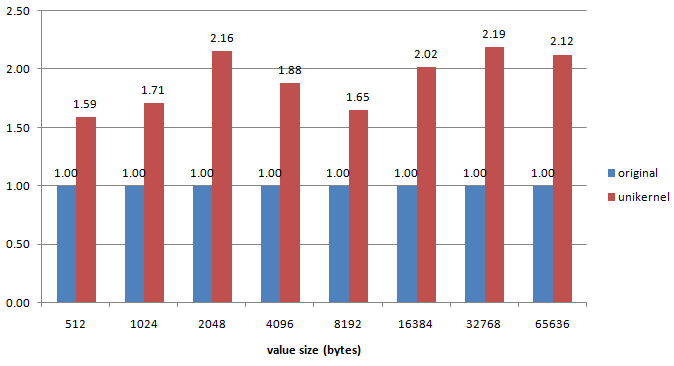
\includegraphics[width=\textwidth]{pictures/secondBenchmarkResults2.PNG}
  \caption{Ποσοστιαία σχέση αυθεντικής \en{utmem} και \en{unikernel utmem} κανονικοποιημένη ως προς
  την αυθεντική}
  \label{fig:original-unikernelPercentage}
\end{figure}

Υπάρχει μια εγγενής ασυμμετρία στα δυο συστήματα που μελετάμε καθώς πρόκειται
για δύο διαφορετικής σχεδίασης και πολυπλοκότητας εικονικές μηχανές. Η εικονική μηχανή μέσα
στην οποία εκτελείται η αυθεντική \en{utmem} διαθέτει διαφορετικό υποσύστημα δικτύου, ενώ εκτελεί παράλληλα
και άλλες διεργασίες εντός της. Ταυτόχρονα, το πλεονέκτημα της \en{unikernel} έκδοσης,
είναι πως χρειάζονται λιγότερες αντιγραφές του \en{value} από το επίπεδο του
\en{Redis} μέχρι και το \en{backend}, το οποίο είναι κοινό και για τις δύο εκδόσεις, ενώ παράλληλα απουσιάζει και η
ανάγκη για \en{context switch}. Αυτή η σχεδιαστική διαφορά εξηγεί την αύξηση της απόδοσης όσο μεγαλώνει το \en{value size}.
Το \en{unikernel} περιβάλλον, προσφέρει ένα σαφές πλεονέκτημα στην ταχύτητα εξυπηρέτησης
των αιτημάτων, το οποίο δείχνει πως αυτές οι δύο τεχνολογίες συνεργάζονται αρμονικότατα.
\newline

Για να εξακριβώσουμε την επιτάχυνση που προσφέρει το \en{Rumprun framework} σε σχέση με
ένα παραδοσιακό \en{VM} συγκρίναμε την εντολή \en{set} του \en{Redis}, τόσο σε \en{unikernel}
περιβάλλον όσο και σε παραδοσιακό \en{VM}, όπως και πριν δηλαδή.
Θεωρούμε πως δίνει μια καλή ποιοτική ένδειξη, καθώς η διαδικασία εξυπηρέτησης της συγκεκριμένης εντολής είναι η ίδια
και στις δύο περιπτώσεις. Το αποτέλεσμα φαίνεται στην εικόνα \ref{fig:original-unikernelSet}. Η συμπεριφορά ταιριάζει με την συμπεριφορά που παρατηρείται
για τα \en{utmem commands}, όπως και αναμένονταν. Φαίνεται πως κατά μέσο όρο, για την περιοχή μεγεθών
που μελετάμε το \en{Rumprun} εμφανίζει περίπου διπλάσιες επίδοσεις σε σχέση με τα συμβατικό \en{VM}.


\begin{figure}[h]
  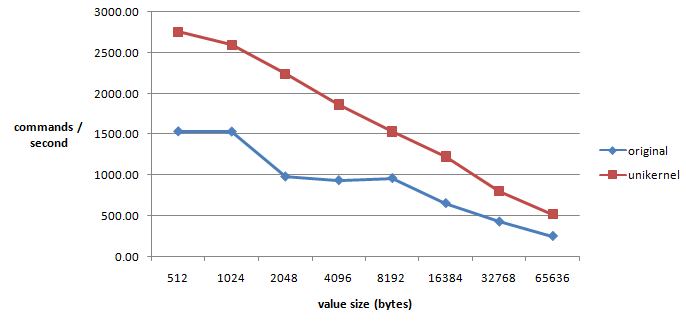
\includegraphics[width=\textwidth]{pictures/secondBenchmarkResults3.PNG}
  \caption{Επίδοση \en{set} εντολής, μεταξύ \en{unikernel} και συμβατικού περιβάλλοντος}
  \label{fig:original-unikernelSet}
\end{figure}




\section{Σχολιασμός}

Από το παραπάνω προκύπτει το εξής ενδιαφέρον συμπέρασμα. Με
χρήση της \en{utmem}, και του \en{Rumprun unikernel framework}, είναι
δυνατόν να εκτελούνται σε εικονοποιημένο περιβάλλον \en{unikernels},
στα οποία αρχικά δίνεται ελάχιστη μνήμη. Στην περίπτωση
του \en{Redis} αρκούν μόνο 64 \en{mega bytes}. Ο φαινομενικός αυτός περιορισμός,
δεν απαγορεύει να εκτελούνται \en{memory intensive} διεργασίας
ως \en{unikernel}, καθώς τα \en{tmem pools} αποθηκεύουν τα δεδομένα που
κανονικά θα βρίσκονταν στην μνήμη εκτός αυτής. Ουσιαστικά εξασφαλίζεται
αδιάκοπη εκτέλεση των \en{unikernels}, και αποφεύγεται η σπατάλη
μνήμης που εν τέλει δεν χρησιμοποιείται από το \en{unikernel}.
Παράλληλα, μεγιστοποιείται ο αριθμός των \en{unikernel}, και
γενικά των εικονικών μηχανών, που μπορούν να εκτελούνται
παράλληλα σε ένα φυσικό σύστημα ανά μονάδα μνήμης.
\newline

Αυτό που πέτυχε στη αυθεντική εργασία η \en{utmem}\cite{Aimilios}, ήταν να
δώσει στον προγραμματιστή ένα χρησιμότατο εργαλείο.
Προσαρμόζοντας ελαφρώς την συμπεριφορά της εφαρμογής
τους ως προς την διαχείριση της μνήμης κέρδισε σε επιδόσεις
και ταχύτητα, σε σχέση με το να εμπιστεύονταν αποκλειστικά
τα υποσυστήματα διαχείρισης μνήμης (\en{frontswap}). Τώρα,
αυτό το εργαλείο προσφέρεται και στο \en{Rumprun unikernel framework},
στο οποίο το σενάριο έλλειψης μνήμης οδηγεί σε καταστροφικές συμπεριφορές.
\newline

Σημαντικό, επίσης, είναι το γεγονός πως η έκδοση \en{utmem} ως \en{unikernel} έχει
επιδόσεις ανώτερες από τον αυθεντικό μηχανισμό. Η επιτάχυνση που προσφέρει το \en{Rumprun} κρίνεται
ζωτικής σημασίας για εφαρμογές ευαίσθητες στον χρόνο απόδοσης, όπως δείξαμε για μια αποθήκη δεδομένων
όπως το \en{Redis}. Τα οφέλη, συνεπώς, πολλαπλασιάζονται, όχι μόνο ελαχιστοποιούνται οι ανάγκες μας σε μνήμη, αλλά
η απόκριση των εικονικών μηχανών, σε σχέση με αντίστοιχους μηχανισμούς, μεταβάλλεται θετικά.
Συμπεραίνουμε πως ο συνδυασμός \en{utmem} και \en{Rumprun} είναι κάθε άλλο από ασύμφορος ή άκαρπος.


\chapter{Επίλογος}

\section{Σύνοψη}

Συνοψίζουμε τα όσα έχουμε παρουσιαστεί έως τώρα στην παρούσα εργασία στον αναγνώστη.
\newline

Αρχικά, έγινε αναφορά στις νέες τάσεις του τρόπου να εκτελούμε
\en{computational tasks}, και συγκεκριμένα στο \en{cloud computing},
το οποίο είναι το μοντέλο που χαρακτηρίζει την σύγχρονη εποχή
στην ιστορία των υπολογιστών. Αναλύθηκε η εικονικοποίηση, η
τεχνολογία που επιτρέπει την ύπαρξη του \en{cloud computing}, καθώς
και τα δίαφορα είδη της που έχουν προκύψει λόγο της δυσκολίας του
να εικονικοποιηθεί ένα πλήρες υπολογιστικό σύστημα. Κατέστη
σαφες ότι η φιλοσοφία των δημοφιλών λειτουργικών συστημάτων
γεννήθηκε σε μια εποχή απλούστερων συστημάτων και περιορισμένων
πόρων και άρα ότι δεν ταιριάζει τέλεια στο \en{cloud computing}.
Παρουσιάστηκαν, λοιπόν, τα εξής προβλήματα με την εως τώρα
εικονικοποίηση. Το πρώτο που είδαμε, είναι η υπερβολική
πολυπλοκότητα των συμβατικών λειτουργικών συστημάτων και οι
υψηλές απαιτήσεις σε πόρους αναλογικά με τις πλέον απλές
εφαρμογές που φιλοξενούν. Το δεύτερο είναι η μη βέλτιστη
διαχείριση των πόρων, και συγκεκριμένα της υφιστάμενης μνήμης
από τα συμβατικά λειτουργικά συστήματα, όταν αυτά βρίσκονται εντός
εικονικοποιημένων περιβαλλόντων.
\newline

Στη συνέχεια, αναλύθηκαν διάφορες τεχνικές αντιμετώπισης των ανωτέρων προβλημάτων.
Το πρώτο πρόβλημα λύνεται με τα \en{unikernels}, αυτές τις ευέλικτες και απλές
εικονικές μηχανές. Κρίθηκε σκόπιμο να αναλυθούν τα
χαρακτηριστικά αυτών και να αναφερθούν τα διάφορα
\en{frameworks} που υπάρχουν. Ειδικά για το \en{Rumprun
framework}, με το οποίο εργαστήκαμε, η ανάλυση επάνω σε
αυτό ήταν εις βάθος, ως έπρεπε. Για το δεύτερο
πρόβλημα προσφέρονται διάφορες λύσεις, ενώ η προσοχή δόθηκε
στην πτητική μνήμη \en{utmem}, καθώς αναλύθηκε η ιστορία
της και τα χαρακτηριστικά της.
\newline

Τελικά, αποδείχθηκε πως αυτές οι δύο τεχνολογίες μπορούν να
συνδυαστούν άψογα, δημιουργώντας \en{unikernels} με \en{utmem} δυνατότητες.
Με σεβασμό στην φιλοσοφία του \en{Rumprun} και στην σχεδίαση της \en{utmem}, αυτές
οι δύο τεχνολογίες εναρμονίστηκαν άψογα.
Μάλιστα, με βάση τις μετρήσεις πο παρατέθηκαν, η ένωση αυτή
δεν είναι άνευ αξίας, αλλά έχει τέλεια εφαρμογή σε συγκεκριμένα
ενδεχόμενα εκτέλεσης εικονικοποιημένων συστημάτων. Διαπιστώθηκε, δε, πως
η επίδοση του νέου μηχανισμού ανώτερη από αυτή της αυθεντικής υλοποίησης.




\section{Μελλοντικές κατευθύνσεις}


Μέχρι στιγμής, η αδυναμία της έκδοσης \en{utmem} για το \en{Rumprun} είναι πως
ως μηχανισμός αποθήκευσης δεδομένων είναι σχετικά αργός σε σχέση
με την αποθήκευση στη μνήμη της εικονικής μηχανής. Θα ήταν δυνατόν
να βελτιστοποιήσουμε περαιτέρω με διάφορες τεχνικές την χρήση της
\en{utmem} ώστε οι ταχύτητες να πλησιάζουν την \en{in-memory} αποθήκευση των
δεδομένων. Κύρια αδυναμία είναι πως, με βάση την μορφή του μηχανισμού,
απαιτείται ένα \en{hypercall} για κάθε αίτηση \en{utmem}. Ανεμένουμε πως αν
μειώνονταν ο αριθμός των \en{hypercalls} που απαιτούνται θα αυξάνονταν οι
επιδόσεις του μηχανισμού.
\newline

Μια λύση θα ήταν να κρατάμε ένα \en{buffer} μνήμης με δεδομένα, τα οποία
θα μεταφέρονταν στην \en{tmem pool} όταν περνούσαν ένα προκαθορισμένο
μέγεθος. Έτσι δεν θα χρειάζονταν να κάνουμε ένα \en{hypercall} ανά
\en{request}, αλλά θα εκμεταλλευόμασταν \en{bulk-insertions} με μόνο ένα
\en{hypercall}. Επί παραδείγματι, ας φανταστούμε πως ερχονται χίλια
αιτήματα \en{utmem} όπου το καθένα επιθυμεί να αποθηκεύσει δεδομένα
μεγέθους ενός \en{kilo byte}.  Θα μπορούσαμε να κάνουμε μαζική
εισαγωγή όλων αυτών, όταν συμπληρωθεί και το π.χ. χιλιοστό αίτημα
με μόνο ένα \en{hypercall} με δεδομένα μεγέθους χίλια επί ένα
\en{kilobyte} συν ό,τι χρειάζεται για τα κλειδιά, αντί για χίλια «μικρά» \en{hypercalls}.
\newline

Άλλη κατεύθυνση θα ήταν τα δεδομένα να συμπιέζονται εντός του
\en{unikernel}, πριν αποσταλούν στο \en{backend}, ώστε πάλι να μειώνεται
ο αριθμός των απαιτούμενων \en{hypercalls}. Ωστόσο, επειδή η συμπίεση
δεδομένων καταναλώνει σημαντική επεξεργαστική ισχύ, αυτό θα
αφορούσε σενάρια εκτέλεσης όπου ο επεξεργαστής είναι πόρος σε
αφθονία, ενώ η μνήμη σε σχετική έλλειψη. Μάλιστα, θα μπορούσε η
εκάστοτε εφαρμογή που τρέχει ως \en{unikernel}, να εξειδικεύει τον
αλγόριθμο συμπίεσης ώστε να ταιριάζει στο είδος των δεδομένων της καλύτερα.
Η εξειδίκευση αυτή είναι πιο εύκολη από την πλευρά του unikernel, καθώς θεωρητικά ο
προγραμματιστής γνωρίζει την φύση των δεδομένων, ενώ το backend εστιάζει στην αποθήκευση
αφηρημένης μορφής δεδομένων.
\newline

Όσον αφορά \en{use case} με πολλές προσβάσεις στην μνήμη επάνω στα
ίδια δεδομένα, η
αποθήκευση και ανάκτηση των δεδομένων με ένα \en{tmem pool} από
μόνη της μειώνει την απόδοση του συστήματος. Γνωστή και
αποδοτική πλέον λύση
τέτοιων περιπτώσεων είναι η χρήση κρυφών μνημών. Στην περίπτωση
μας θα ήταν η ύπαρξη ενός μικρού \en{memory area} μέσα στο
\en{unikernel}, είτε στο ανώτερο επίπεδο είτε στο
επίπεδο του \en{driver}, στο οποίο να βρίσκονται τα περισσότερα συχνά
ανταλλάξιμα δεδομένα μεταξύ του \en{frontend} και του \en{backend}.
\newline

Αναθεωρώντας ακόμα περισσότερο την φιλοσοφία της \en{utmem}, η
χρήση κάποιου ασύχρονου μηχανισμού επικοινωνίας \en{host} και \en{guest},
και όχι του σύγχρονου \en{hypercall}, θα έλυνε τα προβλήματα που
προέρχονται από το \en{blocking} των αιτημάτων. Βέβαια, αυτό
απαιτεί σημαντικά περισσότερη
προσοχή ως προς την ασφάλεια, την αποφυγή αδιεξόδων (\en{deadlock}),
και την εγγύηση πως τα δεδομένα μας θα είναι πάντα διαθέσιμα
και ασφαλή.
\newline

Τέλος, το γεγονός πως επιτρέψαμε την χρήση της \en{utmem} από
\en{unikernels} στηριζόμενοι στο \en{Rumprun}, δεν σημαίνει πως τα άλλα
\en{frameworks} δεν είναι συμβατά. Ανάλογα με το πόσο εύκολο
ή δύσκολο είναι σε έναν προγραμματιστή να προσθέσει μια
κλήση επόπτη στο \en{framework} που τον ενδιαφέρει, θεωρούμε
πως τόσο εύκολο ή δύσκολο είναι και το \en{porting} της \en{utmem}.
Για παράδειγμα, το \en{mirageOS} αν και σχεδιάστηκε για το
\en{Xen hypervisor}, υποστηρίζει και το \en{KVM} πλέον, οπότε πιθανότατα
η ενσωμάτωση του μηχανισμού της \en{utmem} να είναι
σχετικά εύκολη διαδικασία. Το ίδιο ισχύει για τα
περισσότερα \en{frameworks} που υποστηρίζουν το \en{KVM} ως επόπτη.


%Καλημέρα \cite{wikipediaCloud} \cite{JVM} \cite{Aimilios} \cite{QemuWiki} \cite{VMwarePaper} \cite{wikipediaX86} \cite{unikernelsDef} \cite{tmemXenSummit}
%\cite {paperAimiliou} \cite{riseOfVirtLibOS} \cite{libOSCloud}
%\cite{xenArtofVirt}  \cite{overMirage} \cite{includeOS} \cite{Orestis}  \cite{Charalampos}
%\cite{OSV-optimizing} \cite{solo5} \cite{solo5Monitor}
%\cite{rumprunXen}  \cite{noOSnoProb} \cite{interviewKantee}  \cite{wikiUnikernel} \cite{wikiVirtMemory}
%\cite{tmemNutshell} \cite{KVMhyper} \cite{redis} \cite{redisUni}  \cite{redisAOF}



\bibliographystyle{plain}
\bibliography{bibliography}

\end{document}
